\section{23.10.2023}
\section{BJT}
\subsection{Comportamento statico di un BJT}
Il transistore bipolare npn è costituito da due giunzioni n separate da un mezzo drogato p, viceversa quello pnp.\\

%
\noindent\begin{minipage}{0.7\textwidth}
    Il transistore, in generale, non è simmetrico per geometria e drogaggi e pertanto emettitore e collettore non sono interscambiabili.\\
\end{minipage}
\hfill
\begin{minipage}{0.29\textwidth}\raggedleft
    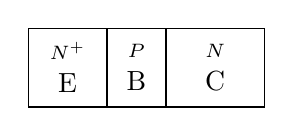
\begin{tikzpicture}
        \draw (0,0) rectangle++(1,1)node[pos=.5,, align=center]{$\scriptstyle N^+$ \\ E}
        rectangle++(0.75,-1)node[pos=.5, align=center]{$\scriptstyle P$ \\ B}rectangle++(1.25,1)node[pos=.5, align=center]{$\scriptstyle N$ \\ C};
    \end{tikzpicture}
\end{minipage}
%
Il BJT npn, essendo composto da due giunzioni pn (e quindi due diodi), può operare in 4 regioni di funzionamento:
\begin{enumerate}
    \item Interdizione
    \item Saturazione
    \item Regione attiva diretta (RAD)
    \item Regione attiva inversa (RAI)
\end{enumerate}
Per capire queste regioni di funzionamento, a seguito vengono mostrate gli schemi base del BJT.\\
\vspace{5mm}
\noindent\begin{minipage}{0.35\textwidth}
    \begin{circuitikz}[american,baseline=(current bounding box.center) ]
    \draw[](-0.5,0.75)node[left]{E} to[short]++(0.5,0);
        \draw (0,0) rectangle++(1.45,1.5)node[pos=.5,, align=center]{$n^+$}
        rectangle++(1,-1.5)node[pos=.5, align=center]{$p$}rectangle++(2.2,1.5)node[pos=.5, align=center]{$n$ };
        \draw(4.65,0.75) to[short]++(0.5,0)node[right]{C};
        %regione EB
        \draw[densely dotted](1.25-0.05,1.5)--++(0,-3.5);
        \draw[densely dotted](1.95-0.1,1.5)--++(0,-3.5);
        %regione BC
        \draw[densely dotted](2.65-0.25,1.5)--++(0,-3.5);
        \draw[densely dotted](3.65-0.25,1.5)--++(0,-3.5);
        %%%%%
        %disegno modello a diodi
        \draw(1.95,-3+.5)node[below]{B} to [short,-*]++(0,1) coordinate(b);
        \draw(b) to [D]++(-1+0.1,0)-|(-0.5,-2+.5)node[left]{E};
        \begin{scope}
        \ctikzset{bipoles/diode/height=0.7, bipoles/diode/width=0.7}
        \draw(b) to [D]++(2,0)-|(4.65+0.3,-2+.5)node[right]{C};
        \end{scope}
        
        %%%%%
        %disegno schema BJT
        \draw(0.9,-3.5) node[left]{E}
        --++(0.5,0) node[npn,anchor=E, rotate=-90, xscale=-1](npn1){}
        (npn1.B)--++(0,-0.5)node[right]{B}
        (npn1.C)--++(0.5,0) node[right]{C};
    \end{circuitikz}
\end{minipage}
\hfill%
\begin{minipage}{0.35\textwidth}\raggedleft
    \begin{circuitikz}[american,baseline=(current bounding box.center) ]
    \draw[](-0.5,0.75)node[left]{E} to[short]++(0.5,0);
        \draw (0,0) rectangle++(1.45,1.5)node[pos=.5,, align=center]{$p^+$}
        rectangle++(1,-1.5)node[pos=.5, align=center]{$n$}rectangle++(2.2,1.5)node[pos=.5, align=center]{$p$ };
        \draw(4.65,0.75) to[short]++(0.5,0)node[right]{C};
        %regione EB
        \draw[densely dotted](1.25-0.05,1.5)--++(0,-3.5);
        \draw[densely dotted](1.95-0.1,1.5)--++(0,-3.5);
        %regione BC
        \draw[densely dotted](2.65-0.25,1.5)--++(0,-3.5);
        \draw[densely dotted](3.65-0.25,1.5)--++(0,-3.5);
        %%%%%
        %disegno modello a diodi
        \draw(1.95,-3+.5)node[below]{B} to [short,-*]++(0,1) coordinate(b);
        \draw(b) to [D,invert]++(-1+0.1,0)-|(-0.5,-2+.5)node[left]{E};
        \begin{scope}
        \ctikzset{bipoles/diode/height=0.7, bipoles/diode/width=0.7}
        \draw(b) to [D,invert]++(2-0.1,0)-|(4.65+0.5,-2+.5)node[right]{C};
        \end{scope}
        %%%%%
        %disegno schema BJT
        \draw(0.9,-3.5) node[left]{E}
        --++(0.5,0) node[pnp,anchor=E,yscale=-1,xscale=-1,rotate=-90](pnp1){}
        (pnp1.C)--++(0.5,0) node[right]{C}
        (pnp1.B)--++(0,-0.5) node[right]{B};
    \end{circuitikz}
\end{minipage}


Interdizione e saturazione sono condizioni limite nelle quali il transistor è un interruttore aperto o chiuso

\subsubsection{Interdizione}
Si ottiene quando le giunzioni base-emettitore e base-collettore sono polarizzate inversamente.\\
In un BJT npn si raggiunge tale condizione se $V_{BE}<0, V_{BC}<0$\\
\textbf{il verso della tensione va dalla zona p alla zona n}.\\
In tali condizioni il transistore è in zona di interdizione.\\
La corrente di emettitore $I_E$ e di collettore $I_C$ sono le correnti inverse di saturazione dei due diodi, e $I_B = - I_E- I_C$. Pertanto tutte le correnti sono trascurabili ( CE è un circuito).

\subsubsection{Saturazione}
Si ottiene quando le giunzioni base-emettitore e base-collettore sono polarizzate direttamente.\\
In un BJT npn si raggiunge tale condizione se $V_{BE}>V_{th}, V_{BC}>V_{th}$ dove $V_{th}$ è la tensione di soglia dei due diodi\\
\textbf{il verso della tensione va dalla zona p alla zona n}.\\
In tali condizioni il transistore è in zona di saturazione.\\
In saturazione, le tensioni delle due giunzioni sono bloccate nell'intorno del valore di $V_{th}$ e la corrente che le attraversa è controllata dal circuito esterno.\\
La tensione di collettore è circa uguale alla tensione di collettore, pertanto si ha che $V_{CE}=V_{C}-V_{E} \approx 0$, questo significa che un circuito collegato ai capi di CE (che preleva $V_CE$) vedrà un circuito aperto.\\

Le altre due condizioni di funzionamento, sono proprie del BJT come dispositivo attivo, si devono analizzare tenendo presente l'interazione fra le due giunzioni

\subsubsection{Regione attiva diretta(RAD)}
Si ottiene quando la giunzione base-emettitore è polarizzata direttamente mentre la giunzione base-collettore è polarizzata direttamente.\\
Questo significa che nella giunzione base emettitore si ha iniezione di elettroni dall'emettitore alla base e iniezione di lacune dalla base all'emettitore.\\
Ora dobbiamo studiare due casi che si possono verificare al variare dello spessore della base $W_B$:\\

Se $W_B$ è molto maggiore della lunghezza di diffusione degli elettroni nella base si dice che le giunzioni BE e BC sono disaccoppiate tra loro.\\
In questa situazione gli elettroni in eccesso iniettati dall'emettitore nella base si ricombinano completamente nella base stessa, ossia non raggiungono la giunzione base-collettore.\\
Tutta la corrente di emettitore fluisce nella base la giunzione base-collettore, polarizzata inversamente, è attraversata dalla sola corrente di saturazione.\\

Se $W_B$ è molto minore della lunghezza di diffusione dei portatori minoritari iniettati nella base, $L_{n,B}$ per un npn.\\
In questo caso la maggior parte dei portatori iniettati non si ricombina, ma diffonde fino alla giunzione base-collettore, dove è catturata dal campo elettrico della regione di svuotamento associata alla giunzione base collettore e raccolta dal collettore.\\
l'interazione tra gionzione BE e BC si chiama effetto transistor.\\
In tale regione l'emettitore emette portatori attraverso la base del collettore, che i raccoglie; una piccola parte di tali portatori si ricombina nella base, dando luoco ad una corrente di lacune nella base.Si ha quindi:

\begin{align}
    |I_C| &\approx |I_E|
\end{align}
Ossia
\begin{align}
    |I_C| &=\alpha|I_E|
\end{align}
con $\alpha \leq 1$. pertanto:
\begin{align}
    |I_B|= |I_E|-|I_C|&=\dfrac{1-\alpha}{\alpha}|I_C|
\end{align}
%
ponendo $\beta=\dfrac{1-\alpha}{\alpha}$, si ha:
\begin{align}
    |I_C| &=\beta|I_B|
\end{align}
dove $\beta \gg 1$.\\
Piccole variazioni di corrente in base causano forti variazioni della corrente di collettore e di emettitore: il BJT in regione attiva diretta è un amplificatore di corrente pilotato in corrente

\subsubsection{Regione attiva inversa(RAI)}
non è di mio interesse, è inutile e meno efficiente del RAD. Se necessario leggere Ghione pagina 536.
\cleardoublepage

\subsection{Parametri caratteristici in RAD}
Indico con $F_n$ il flusso di elettroni attraverso una superficie (numero di elettroni per unità di tempo che attraversa la superficie), con $F_h$ il flusso di lacune.
Le relative correnti saranno $I_n=-qF_n$ e $I_h=qF_h$.\\
\begin{figure}[h]\centering
    \begin{tikzpicture}[scale=0.75]
        \draw(0,4) rectangle++(4.5,-4) rectangle++(3,+4) rectangle++(4.5,-4); %rettangolo di dimensione 12,4

        % disegno zona svuotamento EB
        \draw[pattern=north east lines, pattern color=gray](4.25,0) rectangle (4.75,4);
        % disegno zona svuotamento BC
        \draw[pattern=north east lines, pattern color=black](6,0) rectangle (9,4);
        
        %disegno corrente elett da E a B
        \coordinate[] (anEB) at (3.5,3);
        \coordinate[] (bnEb) at (5.15,3);
        \node[single arrow, draw=blue, very thick, fill=white,
        minimum width = 10pt, single arrow head extend=3pt,
        inner xsep=0pt,
        fit=(anEB) (bnEb)] {}; % length of arrow
        %label
        \node at (2.8,3) [blue]{$F_{nEB}$};

        %disegno corrente elett da B a C
        \coordinate[] (anBC) at (5.7,3);
        \coordinate[] (bnBC) at (9.35,3);
        \node[single arrow, draw=blue, very thick, fill=white,
        minimum width = 10pt, single arrow head extend=3pt,
        inner xsep=0pt,
        fit=(anBC) (bnBC)] {}; % length of arrow
        %label
        \node at (10.25,3) [blue]{$F_{nBC}$};

        %disegno corrente lacune da B a E
        \coordinate[] (ahBE) at (3.5,1);
        \coordinate[] (bhBE) at (5.25,1);
        \node[single arrow,draw=red, very thick, fill=white,
        minimum width = 10pt, single arrow head extend=3pt,
        inner xsep=0pt,rotate=180,
        fit=(ahBE) (bhBE)] {}; % length of arrow
        %label
        \node at (2.65,1) [red]{$F_{hBE}$};

        %altre correnti da B a C
        \draw[{Triangle[width=8pt,length=6pt]}-, line width=3pt](5.5,1.5) --++ (4.25, 0);
        %label
        \node at (10.45,1.5) [black]{$F_{hBC0}$};
        \draw[-{Triangle[width=8pt,length=6pt]}, line width=3pt](5.5,0.5) --++ (4.25, 0);
        %label
        \node at (10.45,0.5) [black]{$F_{nBC0}$};

        %ingressi e correnti di ingresso
        \draw [fill=gray!40!black] (-0.15,0.5) rectangle++ (0.15,3);
            \draw[thick] (-1,2) node[left]{E}
                 to [short,*-]++(1,0);
            \draw[>=latex,->] (-1,1.8)--++(0.75,0) node[anchor=north east]{$I_E$};
            
        \draw [fill=gray!40!black] (12,0.5) rectangle++ (0.15,3);
            \draw[thick] (13,2) node[right]{C}
                 to [short,*-]++(-1,0);
            \draw[>=latex,->] (13,1.8)--++(-0.75,0) node[anchor=north west]{$I_C$} ;
                 
        \draw [fill=gray!40!black] (5,-0.15) rectangle++ (2,0.15);
            \draw[thick] (6,-1.15) node[right]{B}
                 to [short,*-]++(0,1);
            \draw[>=latex,->] (5.8,-1.15)--++(0,0.75) node[anchor= north east]{$I_B$};

        %label NPN
        \draw[densely dotted](4.5,4)--++(0,1);
        \draw[densely dotted](7.5,4)--++(0,1);
        \node at (2.25,4.5)[]{N};
        \node at (6,4.5)[]{P};
        \node at (9.75,4.5)[]{N};
        
    \end{tikzpicture}
\caption{Flusso di elettroni e lacune in un BJT npn in RAD. Le regioni svuotate non sono proporzionalmente corrette ma è per dare l'idea}
\label{fig:Flusso di elettroni e lacune in un BJT npn in RAD}
\end{figure}

All'interno del BJT npn in RAD si distinguono diverse componenti di flusso delle particelle:
\begin{itemize}
    \item $F_{nEB}$ è il flusso di elettroni iniettati dall'emettitore alla base a causa della polarizzazione diretta della giunzione B-E;
    
    \item $F_{hBE}$ è il flusso di lacune iniettate dalla base all'emettitore a causa della polarizzazione diretta della giunzione base emettitore. \textbf{è una componente indesiderata}/parassita perchèncontribuisce all'aumento di $I_B$ ma non all'aumento di $I_C$. In altre parole: il contributo di  $I_E$ che si crea grazie ad $F_{hBE}$ non raggiunge il collettore, ma è raccolta nell'emettitore. pertanto una variazione di questo flusso causata dalla corrente $I_B$ non influisce sulla corrente di collettore.
    
    \item $F_{nBC}$ è il flusso di elettroni che, attraversata la base, raggiungono la giunzione base-collettore. Se la base è sottile rispetto alla lunghezza di diffusione degli elettroni, la maggior parte degli elettroni non si ricombina nella base con le lacune ma viene raccolta dal collettore.\\
    lE LACUNE CHE SI RICOMBINANO CON GLI ELETTRONI INIETTATI NELLA BASE danno luogo alla sola componente utile della corrente di base
    \begin{ricevimento}
        spiegare ultima frase
    \end{ricevimento}
    \item $F_{nBC0}$ e $F_{hCB0}$ sono gli elettroni e le lacune che attraversano la giunzione B-C quando l'emettitore è aperto. Sono quindi le componenti della piccolissima corrente inversa di saturazione della giunzione B-C.\\
    Sono componenti parassite perchè non pilotate dalla corrente di base ed hanno un valore trascurabile in regione attiva diretta ma divengono le componenti principali in regione attiva inversa (che non si studia).
    
\end{itemize}
Tenendo presente che le correnti sono considerate entranti (figura \ref{fig:Flusso di elettroni e lacune in un BJT npn in RAD}), si ha:
allora il flusso totale di cariche che entra nell'emettitore sarà:
mentre il flusso totale di cariche che entra nel collettore
\begin{align}
F_E &= F_{nEB}-F_{hBE}\\
    F_C &= -F_{nBC}-F_{nBC0}+F_{hCB0}
\end{align}
\begin{ricevimento}
    Fe ed Fc li devo moltiplicare per +q o -q?
\end{ricevimento}
per ottenere le cariche moltiplico tutto per q, ricordando che le lacune hanno segno positivo mentre gli elettroni hanno segno negativo.:
\begin{align}
I_E &= (-q)F_{nEB}+q(-F_{hBE})\\
    I_C &= (-q)(-F_{nBC})+(-q)(-F_{nBC0})+qF_{hCB0}
\end{align}
Ovvero:
\begin{align}
I_E &= -qF_{nEB}-qF_{hBE}\\
    I_C &= qF_{nBC}+qF_{nBC0}+qF_{hCB0}
\end{align}
Dove chiamo $I_{CB0}=qF_{nBC0}+qF_{hCB0}$ la corrente inversa di saturazione della giunzione base collettore (è quella che si misura fra C-B quando E è aperto) ed è importante perchè il contributo di corrente di elettroni inversa si mescola con quello che arriva all'emettitore.\\ allora:
\begin{align}
    I_C &= qF_{nBC}+I_{CB0}
\end{align}
   
Dando un'occhiada al modello a diodi di un BJT npn, si nota come le correnti possano essere calcolate dalla legge di Khirchoff:
\begin{align}
    I_B &= -I_E-I_C
\end{align}
ossia:
\begin{align}
     I_B &= qF_{hBE}+\-I_{CB0}
\end{align}
Dove $qF_{nEB}-qF_{nBC}$ rappresenta il numero di elettroni che si ricombinano in base.
\begin{psbox}
\textbf{La corrente di base nasce per mantenere l'eccesso di continuo rifornimento di lacune che si ricombinano con gli elettroni di EB}
    Per questo si dice spesso che il BJT è pilotato in corrente  ma non è appropriato usare questa frase!\\
    il transistor è pilotato in tensione, ma le giunzioni hanno una forte variazione in corrente e questo implica che serve molta precisione per regolare la corrente , quindi spesso si pilota in corrente
    \begin{ricevimento}
        Spiegare meglio?
    \end{ricevimento}
\end{psbox}
Adesso definiamo dei parametri importanti:
\begin{itemize}
    \item Efficienza di emettitore  
    \begin{equation}
        \label{eqn:efficienza di emettitore}
        \gamma = \dfrac{F_{nEB}}{F_{nEB}+F_{hBE}}
    \end{equation}
    è il rapporto tra la corrente associata ai portatori (elettroni) iniettati dall'emettitore nella base e le correnti totali che attraversano la giunzione Base-Emettitore. Idealmente $\gamma=1$ ma, realisticamente parlando sarebbe $\gamma < 1$

    \item Fattore di trasporto in base 
    \begin{equation}
        \label{eqn:fattore di trasporto in base}
        b=\dfrac{F_{nBC}}{F_{nEB}}
    \end{equation}
    è il rapporto tra la corrente di elettroni che dalla base va all'emettitore e la corrente di elettroni che dall'emettitore va dentro la base.\\
    Idealmente dovrebbe essere 1.
    \item amplificazione di corrente a base comune $\alpha$
    \begin{equation}
        \label{eqn:amplificazione di corrente a base comune}
     \alpha = \dfrac{F_{nBC}}{F_{nEB}+F_{hBC}} = b \gamma
    \end{equation}
    è espresso come rapporto tra la corrente di collettore e quella di emettitore nel caso in cui non ci siano correnti di saturazione inversa.\\
    idealmente è 1 ma realisticamente è minore di 1.\\

    Siccome è chiamato amplificatore sembra difficile che sia un parametro minore di 1.Non si ha amplificazione assumento come ingresso $I_E$ e come uscita $I_C$. l'amplificazione i corrente è in realtà $\beta$ (che è descritto dopo) assumento $I_C$ come uscita ed $I_B$ come corrente di ingresso
    
    \item amplificazione di corrente a emettitore comune $\beta$
    \begin{equation}
        \label{eqn:amplificazione di corrente a emettitore comune}
        \beta = \dfrac{\alpha}{1-\alpha}
    \end{equation}
\end{itemize}
Tenendo presente dal'equazione \ref{eqn:fattore di trasporto in base} che:
 \begin{equation}
     F_{nBC}=b \ F_{nEB}
 \end{equation}
e dall'equazione \ref{eqn:efficienza di emettitore} che:
\begin{equation}
    F_{nEB}+F_{hBE}=\dfrac{F_{neB}}{\gamma}
\end{equation}
si ha:
\begin{align}
    I_E &= -qF_{hBE}-qF_{nEB}= - \dfrac{-qF_{nEB}}{\gamma}\\
    I_C &= qbF_{nEB}+I_{CB0}
\end{align}

da cui, eliminando $F_{nEB}$:

\begin{equation}
    I_C=-\gamma b I_E + I_{CB0}\label{eq:formula Ic ebers-moll}
\end{equation}

Adesso, ricordo che $\alpha = \gamma b $ e che $alpha \approx 1$ allora la corrente $I_C$ si può approssimare come
\begin{equation}
    I_C=-\gamma b I_E + I_{CB0} \approx - \alpha I_E
\end{equation}

considerando quindi la legge di Khirchoff, si può portare in funzione di $I_B$:
\begin{align}
    I_B&=-I_E-I_C \\
    I_C&= \dfrac{\alpha}{1-\alpha}I_B + \dfrac{1}{1-\alpha}I_{CB0} 
\end{align}
    Usando l'equazione (\ref{eqn:amplificazione di corrente a emettitore comune}):
\begin{align}
    I_C&= \beta I_B + (1+\beta)I_{CB0}
\end{align}

Quindi la corrente di collettore è composta da una corrente di saturazione inversa amplificata di $\beta +1$. Questo rappresenta un problema visto che $\beta$ è alto e $I_{CB0}$ dipende dalla temperatura e provoca il \textbf{ runaway termico} :
se T aumenta, $I_{CB0}$ aumenta quindi $I_C$ aumenta facendo aumentare la potenza dissipata e di conseguenza la temperatura. E' un cane che si morde la coda.\\

\begin{psbox}
    Per risolvere questo problema si può mettere una reisstenza di emettitore o base che realizza un feedback negativoche riduce la tensione Vbe.
    figure e pro e contro delle due configurazioni
\end{psbox}

\cleardoublepage
\subsubsection{BJT dal punto di vista delle bande}
Come funziona in linea generale:
In condizionid i equilibrio si instaura, tra le giunzioni base-emettitore e base-collettore, una potenziale di giunzione.

\begin{figure}[hbt!]
    \centering
    \begin{tikzpicture}
    \begin{scope}[scale=1.25]
        \draw[](-0.5,0.75)node[left]{E} to[short]++(0.5,0);
        \draw (0,0) rectangle++(1.45,1.5)node[pos=.5,, align=center]{$n^+$}
        rectangle++(0.75,-1.5)node[pos=.5, align=center]{$p$}
        rectangle++(2.2+0.3,1.5)node[pos=.5, align=center]{$n$ };
        \draw(4.7,0.75) to[short]++(0.5,0)node[right]{C};
        %regione EB
        \draw[densely dotted](1.3,1.5)--++(0,-10);
        \draw[densely dotted](1.65,1.5)--++(0,-10);
        %regione BC
        \draw[densely dotted](2.15,1.5)--++(0,-10);
        \draw[densely dotted](3.15,1.5)--++(0,-10);
        %diagramma a bande in equilibrio
        \draw (0,-2+0.5)--(1.1,-2+0.5) to [out=0, in=180](1.75,-1+0.5)--(2.15,-1+0.5)to [out=0, in=180](3.15,-2+0.5)--(4.7,-2+0.5);
        \draw (0,-3.1+0.5)--(1.1,-3.1+0.5) to [out=0, in=180](1.75,-2.1+0.5)--(2.15,-2.1+0.5)to [out=0, in=180](3.15,-3.1+0.5)--(4.7,-3.1+0.5);
        %diagramma a bande NON in equilibrio
        \draw (0,-4.5)--(1.1,-4.5) to [out=0, in=180](1.75,-4)--(2.15,-4)to [out=0, in=180,distance=0.6 cm](3.15,-6)--(4.7,-6);
        \draw (0,-5.6)--(1.1,-5.6) to [out=0, in=180](1.75,-5.1)--(2.15,-5.1)to [out=0, in=180,,distance=0.6 cm](3.15,-7.1)--(4.7,-7.1);
        %livelli di fermi
        
        %label diffusione elettroni
        \draw[-latex](1,-3.25)--++(0.75,0)node[align=center, anchor=south east]{Diffusione \\ elettroni};
        %label deriva elettroni
        \draw[-latex](2,-3.25)to[out=0, in=110]++(1.5,-2)node[align=center, anchor=south west]{deriva \\ elettroni};
    \end{scope}

    %diagramma a bande non in equilibrio
    \end{tikzpicture}
    \caption{Caption}
    \label{fig:enter-label}
\end{figure}
Se poi supponiamo di avere un BJT in RAD, avrò la giunzione BE attiva e la giunzione BC spenta risultando nel grafico in figura (b).\\
Gli elettroni dell'emettitore si diffondono per diffusione verso la base mentre si spostano dalla base verso il collettore per effetto deriva. 
una volta che gli elettroni hanno raggiunto la regione di svuotamento B-C vengono attratti dal compo elettrico nella direzione di C(scivolo potenziale). \\
modificando Vbe regolo la popolazione di elettroni in base (e quindi quelli che arriveranno al collettore se la base è corta)e quindi la raccolta. ma Vbc in prima approssimazione non si modifica. si hanno delle correnti costanti in funzione di vbc, le correnti Ie circa= I applicata.
Quindi per far si che vi sia corrente in uscita si deve rendere nulla la corrente la correnteproveniente dal C nella B (mandando in cut off la giunzione corrispondente) altrimenti le correnti si annullerebbero
\begin{figure}[hbt!]
    \centering
    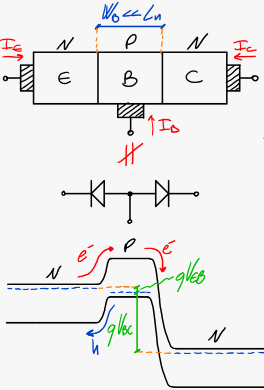
\includegraphics{Immagini_Micro&Nano/Imm_3_Transistor_BJT/BJTNPN.png}
    \caption{Diagramma a bande di un BJT npn}
    \label{fig:Diagramma a bande di un BJT npn}
\end{figure}
 \cleardoublepage
Gli elttroni dall'emettitore passano nella base grazie al potenziale $V_{EB}$ che riduce la barriera di potenziale su E-B.\\
Questi elettroni si ritroveranno nella base ed in parte si ricombineranno con le lacune ma, grazie al fatto che la base è corta, molti riescono ad arrivare alla regione di svuotamento B-C che è praticamente uno scivolo (grazie alla presenza di $V_{BC}$ che dirige/lancia gli elttroni e li fà entrare in C).\\
Questo processo è tanto più efficacie quanto più la base è sottile. Inoltre, si capisce che, regolando la $V_{BE}$ regolo anche il numero di elettroni iniettati e quindi regolo la corrente di emettitore.
se la base è corta allora tale corrente sarà la $I_C$ cioè la corrente di soglia. E' importante marcare che ho fatto una grossa approssimazione: all'aumentare di $V_{BC}$,  la $I_C$ rimane costante.
\begin{psbox}
Se agisco sulla qVbc gli elettroni una volta raggiunta la I\_c cadono comunque in C: 
\begin{ricevimento}
    spiegare
\end{ricevimento}
    \begin{center} 
       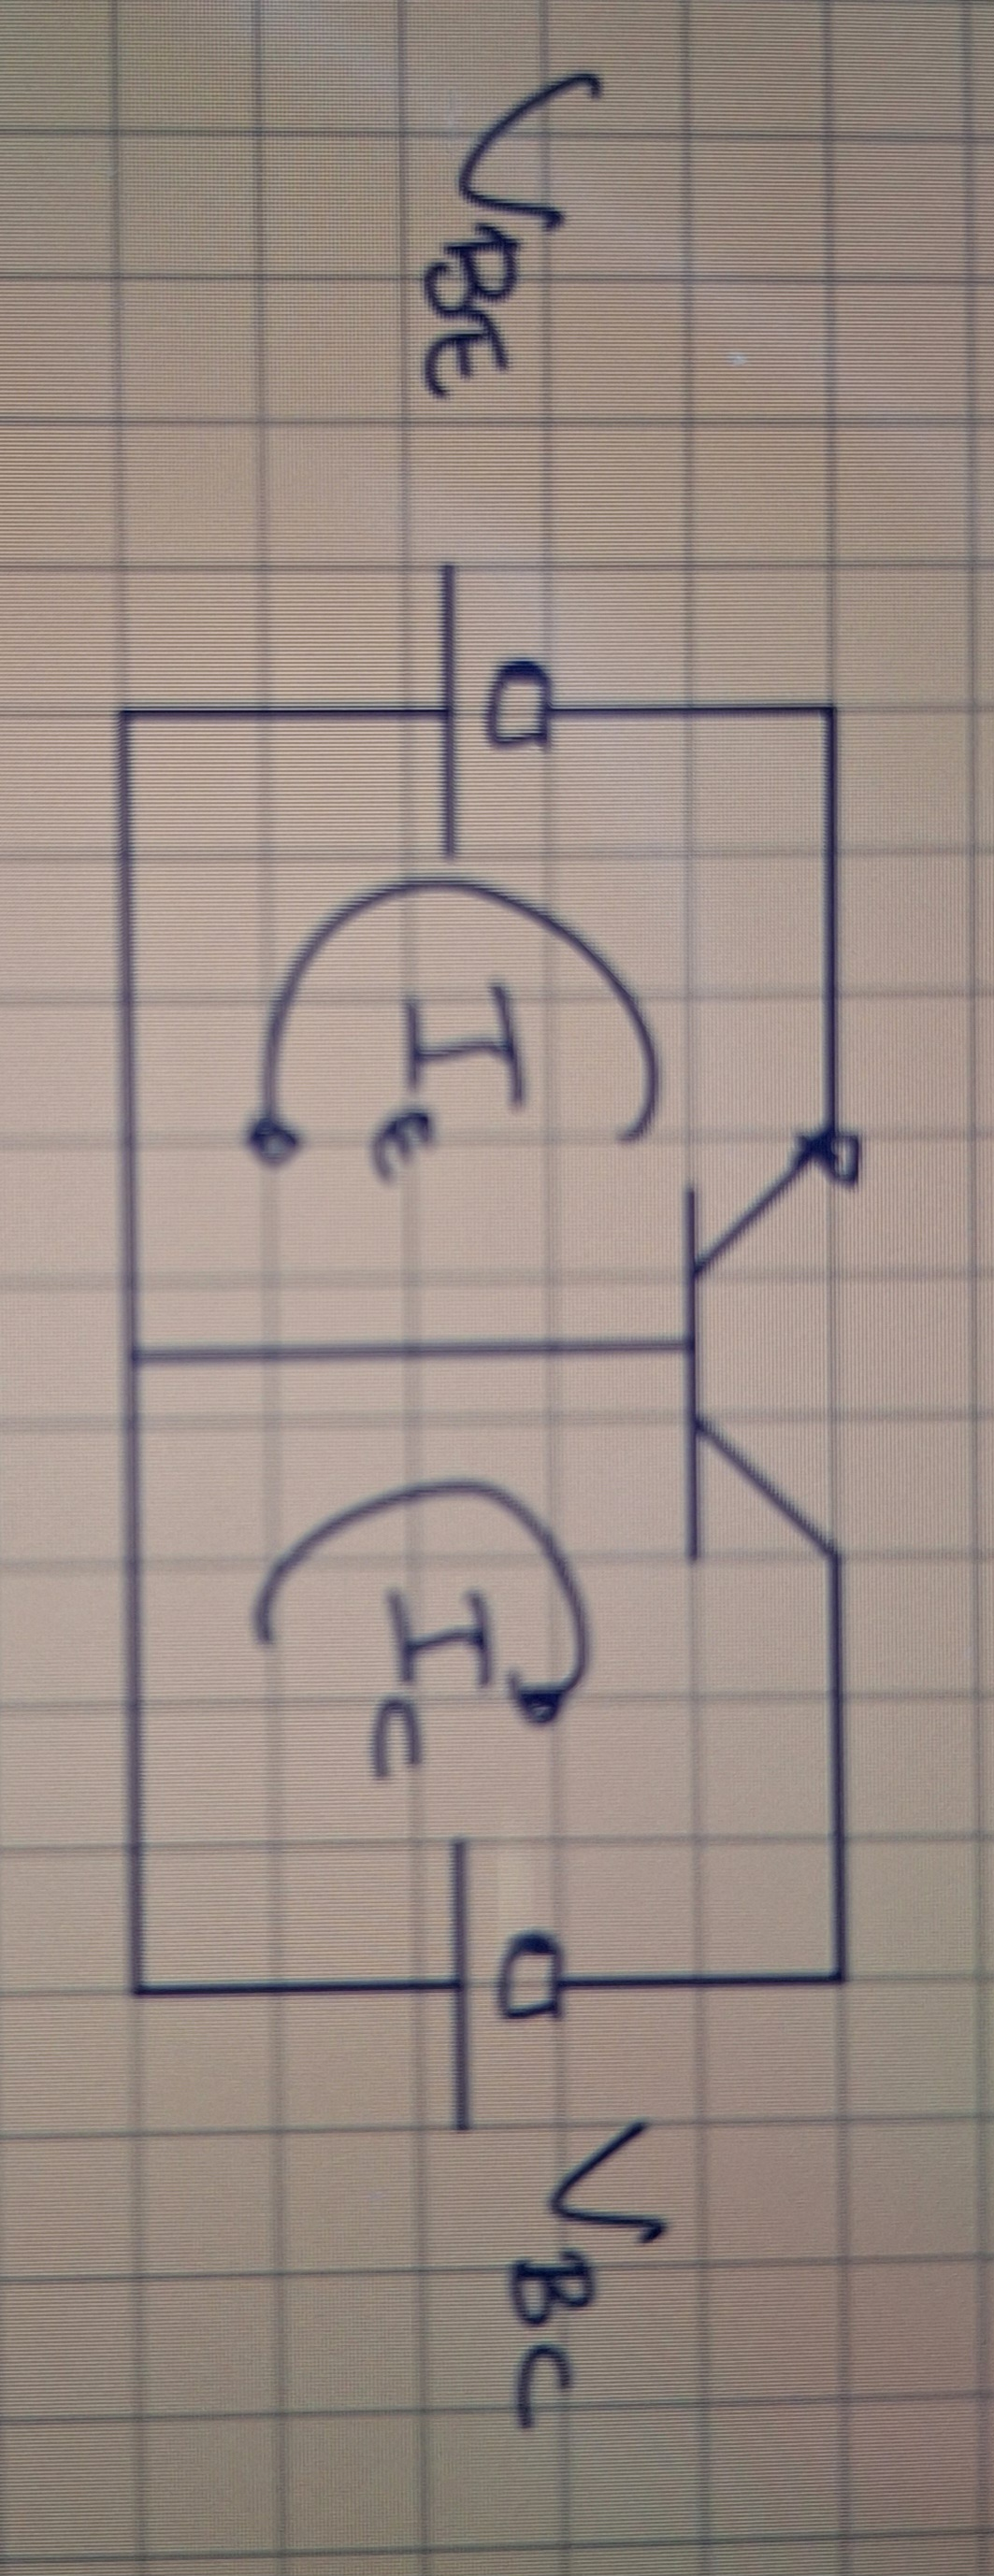
\includegraphics[width=0.25\textwidth,angle=90]{Immagini_Micro&Nano/Imm_3_Transistor_BJT/polarizzazBJTRAD.png}
       \vspace{5mm}
        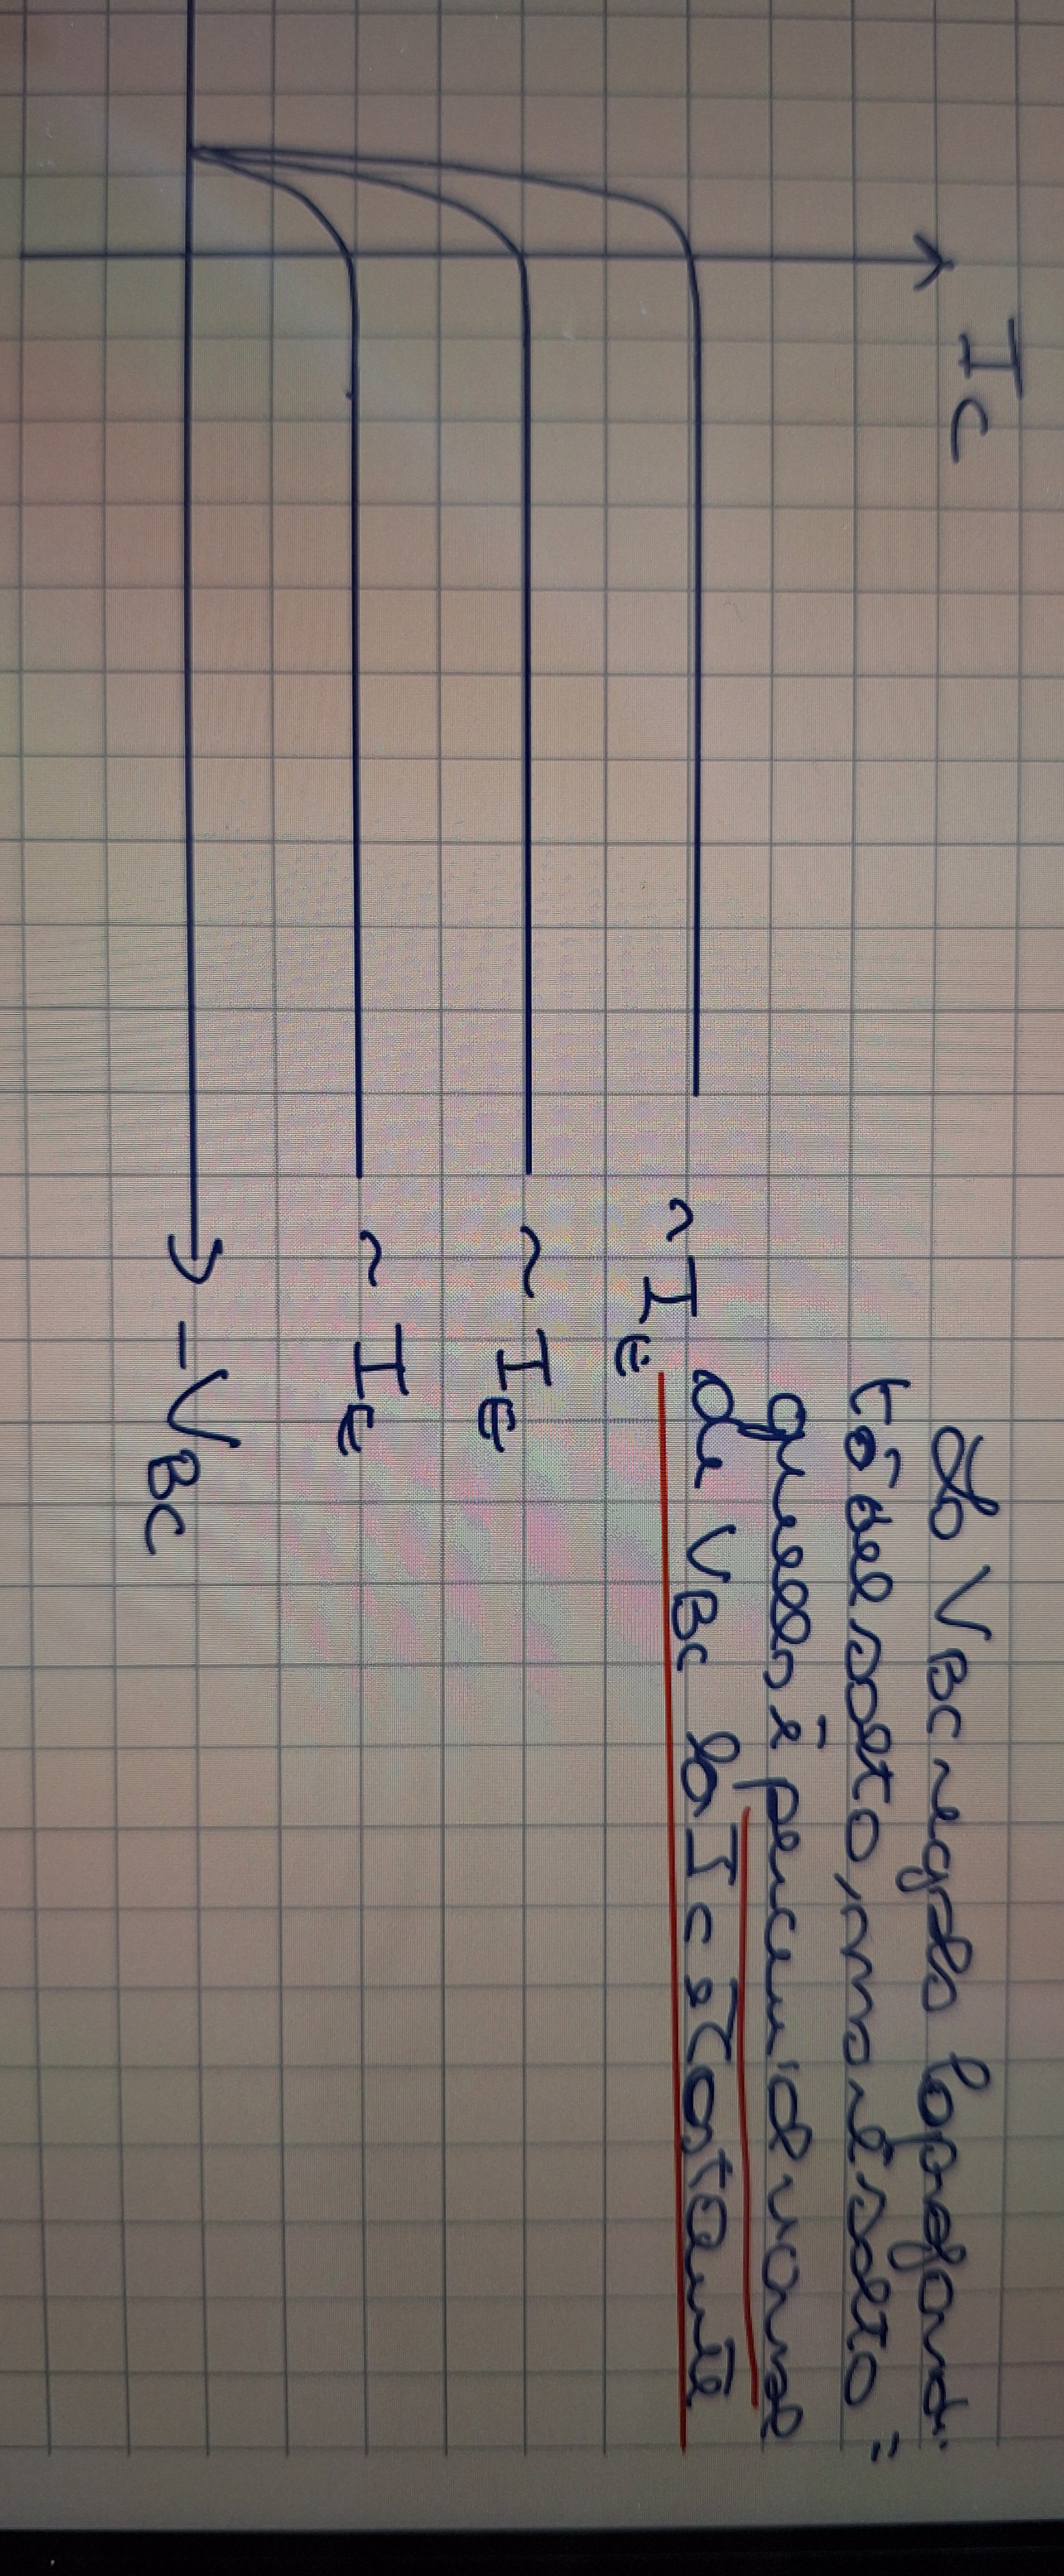
\includegraphics[width=0.25\textwidth,angle=90]{Immagini_Micro&Nano/Imm_3_Transistor_BJT/caratteristicaBJTRAD.png}
    \end{center} 
\end{psbox} 

Ignorando le zone di svuotamento avrò un profilo dei portatori minoritari come in figura:
\begin{figure}[hbt!]
    \centering
    \begin{tikzpicture}[scale=1]
        \draw(0,0)--++(12,0);
        \draw(4,0)--++(0,3.5)node[above]{$X_E$};
        \draw(8,0)--++(0,3.5)node[above]{$X_C$};
        
        \draw[dashed](0,0.5)--++(4,0);
        \draw[dashed](4,0.5)--++(4,0);
        \draw[dashed](8,0.5)--++(4,0);

        \node at (2,3.5)[]{N};
        \node at (6,3.5)[]{P};
        \node at (10,3.5)[]{N};

        %grafico rosso
        \draw[very thick,red] (4,2.5) to [out=240,in=1] (0,0.55) ;
        % label formula
        \node at (4,2.8)[left]{$pn_0e^{\dfrac{V_{be}}{V_T}}$};
        \draw[very thick,red] (4,2.5).. controls (5,1.5) and (5.7,1.55) .. (6,1.45);
        %cerchio
        \node[circle,fill=black,inner sep=0pt,minimum size=4pt] at (4,2.5)[]{};
        % label formula
        \node at (4,2.8)[right]{$np_0e^{\dfrac{V_{be}}{V_T}}$};
        \draw[very thick,red] (6,1.45) to [out=-5,in=120] (8,0) ;
         %cerchio
        \node[circle,fill=black,inner sep=0pt,minimum size=4pt] at (8,0)[]{};
        % label formula
        \node at (6.5,-0.32)[right]{$np_0e^{\dfrac{V_{be}}{V_T}}$};
        \draw[very thick,red] (8,0) to [out=17,in=180] (12,0.45) node[right,black]{$pn_0$};
       
        % label formula
        \node at (8,-0.32)[right]{$pn_0e^{\dfrac{V_{bc}}{V_T}}$};

        %carica
         \draw[pattern=north east lines, pattern color = gray] (4,0)--(4,2.5).. controls (5,1.5) and (5.7,1.55) .. (6,1.45)to [out=-5,in=120] (8,0)--(4,0); 
         \node at (5.5,1)[] {$\textbf Q_B$};
         

         %freccie e label
         \draw[>=latex, <->] (0,-0.25)--(3.9,-0.25); \node at (2,-0.25)[anchor=north]{$W_E$};
         \draw[>=latex, <->] (4.1,-0.25)--(7.9,-0.25); \node at (6,-0.25)[anchor=north]{$W_B$};
         \draw[>=latex, <->] (8.1,-0.25)--(12,-0.25); \node at (10,-0.25)[anchor=north]{$W_C$};

         \draw[>=latex, <-,blue] (4,-0.1)--++(0,-0.5) node [anchor=north,blue]{$on$};
         \draw[>=latex, <-,blue] (8,-0.1)--++(0,-0.5) node [anchor=north,blue]{$off$};
         
    \end{tikzpicture}
    \caption{Caption}
    \label{fig:enter-label}
\end{figure}

Ora ricordo che la corrente è data dalla la variazione di carica nel tempo.\\
Prima di continuare  definisco due parametri di tempo che serviranno per studiare la variazione di carica nella base:
\begin{itemize}
    \item $\tau_t$: tempo di transito in base. E' il tempo medio impiegato dai portatori minoritari (elettroni iniettati nella base dall'emettitore) per attraversare la zona neutrale della base e raggiungere il limite della regione di svuotamento della giunzione base-collettore. 
    \item $\tau_0$: tempo di vita medio dei portatori minoritari nella base ($\tau_n$ per un npn, $\tau_h$ per un pnp). 
\end{itemize}
%
Le cause che provocano la variazione nel tempo della carica mobile all'interno della base sono due.\\
La prima è dovuta al transito dei portatori dalla giunzione emettitore-base verso la giunzioene base-collettore:
\begin{equation}
    \left.\dfrac{dQ_B}{dt}\right|_t= -\dfrac{Q_B}{\tau_t}
\end{equation}
La seconda causa si riferisce al fenomeno della ricombinazione che ha effetto sulle cariche mobili iniettate nella base dall'emettitore:
\begin{equation}
    \left.\dfrac{dQ_B}{dt}\right|_R= -\dfrac{Q_B}{\tau_0}
\end{equation}
Perché il transistore funzioni correttamente è necessario che la variazione di carica per effetto della ricombinazione sia molto minore della variazione di. carica per effetto del transito. Infatti si ha, trascurando la $I_{CB0}$: 

\begin{align}
    |I_C|&= -\left.\dfrac{dQ_B}{dt}\right|_t= \dfrac{Q_B}{\tau_t}
    \end{align}
    mentre, trascurando la componente della corrente di base dovuta alle lacune if1iettate nell'emettitore (ossia ponendo $\gamma \approx 1$): 
\begin{align}
    |I_B|&= -\left.\dfrac{dQ_B}{dt}\right|_R= \dfrac{Q_B}{\tau_0}
\end{align}

\begin{psbox}
    ricordo, dall'equazione di continuità che \[ \dfrac{dQ}{dt}= \nabla \cdot J\]. Nel caso monodimensionale esso si traduce in \[\dfrac{dQ}{dt}=\dfrac{dJ}{dx}\]
\end{psbox}
nell'immediato 
\begin{equation}
    \beta=\dfrac{I_C}{I_B} \approx \dfrac{\tau_0}{\tau_T}
\end{equation}
quindi $\beta \uparrow$ se $\tau_0 \uparrow$ e $\beta \downarrow$ se $\tau_T \uparrow$. tuttavia per avere bjt veloce servirà $\tau_0 \downarrow$, ecco che capisco che bisogna fare un compromesso

\subsubsection{Come calcolare Le correnti del BJT  in modo analitico}
Seguirò gli stessi ragionamenti fatti nel caso di giunzione PN ma applicando, più avanti, un'opportuna semplificazione delle correnti di diffusione (in questo caso corrente di lacune).\\
Si parte considerando la corrente di diffusione delle lacune nell'emettitore:
\begin{equation}
    I_{P,D}=-qD_P\dfrac{dp}{dx}
\end{equation}
Dove $D_P$ è la diffusività delle lacune mentre $\frac{dp}{dx}$ indica la variazione spaziale della concentrazione di lacune.\\
E' possibile semplificare il calcolo seguendo due considerazioni:\\
\begin{enumerate}
    \item Innanzitutto, considero la lunghezza dell'emettitore come fosse corta laddove le cariche si diffondono. Questo vuoldire che \textbf{la lunghezza di diffusione delle lacune nell'emettitore è molto minore(maggiore?) della dimensione fisica dell'emettitore($W_E$)}.
la medesima cosa si applica agli elettroni nella base e alle lacune nel collettore. Quindi:
\begin{align}
    Lp_{E} & \ll W_E\\
    Ln_B &\ll W_B \\
    Ln_C &\ll W_C
\end{align}
\item Inoltre, devo ricordare che il terminale sinistro dell'emettitore dovrà essere metallizzato per permettere la connessione con mondo esterno, creando la giunzione Schottky.
La metallizzazione ci costringe a considerare le condizioni a contorno che si formano con il metallo, infatti i portatori minoritari in eccesso, che altrimenti contribuirebbero alla corrente di diffusione, vengono raccolti o bloccati dal metallo, influenzando così le condizioni di contorno e semplificando l'analisi.\\
%
\end{enumerate}


\begin{ricevimento}
    qui mi sono perso
\end{ricevimento}
Detto questo, posso approssimare la concentrazione dei portatori con andamento esponenziale, come se  avessero l'andamento di una retta, consentendomi di semplificare la derivata presente all'interno della $I_{P,D}$.



\begin{figure}[hbt!]
    \centering
    \begin{subfigure}[]{0.49\textwidth}
        \centering
        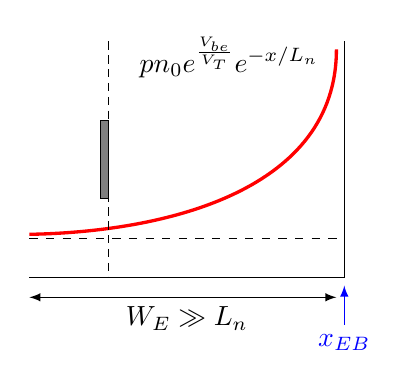
\begin{tikzpicture}[scale=1]
        
            \draw(0,0)--++(4,0);
            \draw(4,0)--++(0,3);
            
            \draw[dashed](0,0.5)--++(4,0);
    
            %grafico rosso
            \draw[very thick,red] (3.9,2.9) to [out=270,in=1] (0,0.55) ;
            % label formula
            \node at (3.8,2.8)[left]{$pn_0e^{\frac{V_{be}}{V_T}}e^{-x/L_n}$};

             %freccie e label
             \draw[>=latex, <->] (0,-0.25)--(3.9,-0.25); \node at (2,-0.25)[anchor=north]{$W_E \gg L_n$};
             \draw[>=latex, <-,blue] (4,-0.1)--++(0,-0.5) node [anchor=north,blue]{$x_{EB}$};

             %metallizzazione
             \draw[densely dashed](1,3)--++(0,-3);
             \draw [fill=gray](1,1) rectangle++(-0.10,1);
        \end{tikzpicture}
        \caption{reale}
        \label{fig:enter-label}
    \end{subfigure}
    %
    \begin{subfigure}[]{0.49\textwidth}
        \centering
        \begin{tikzpicture}[scale=1]
            \draw(0,0)--++(4,0);
            \draw(4,0)--++(0,3);
            
            \draw[dashed](0,0.5)--++(4,0);
    
            %grafico rosso
            \draw[very thick,red] (4,2.5) -- (1,0.55) ;
            % label formula
            \node at (4,2.8)[left]{$pn_0e^{\dfrac{V_{be}}{V_T}}$};
            
            %cerchio
            \node[circle,fill=black,inner sep=0pt,minimum size=4pt] at (4,2.5)[]{};
 
             %freccie e label
             \draw[>=latex, <->] (1,-0.25)--(3.9,-0.25); \node at (2.5,-0.25)[anchor=north]{$W_E \ll L_n$};
             \draw[>=latex, <-,blue] (4,-0.1)--++(0,-0.5) node [anchor=north,blue]{$x_{EB}$};

             %metallizzazione
             \draw[densely dashed](1,3)--++(0,-3);
             \draw [fill=gray](1,1) rectangle++(-0.10,1);
        \end{tikzpicture}
        \caption{approssimato}
        \label{fig:enter-label}
    \end{subfigure}
    
    \caption{Caption}
    \label{fig:enter-label}
\end{figure}
%
La variazione della concentrazione di portatori minoritari nella regione metallizzazione di emettitore fino all'inizio della regione svuotata ($x_{EB}$), può essere calcolata come il semplice rapporto "Base $\cdot$ altezza":
\begin{equation}
    \left. \dfrac{dp}{dx}\right|_{x_{EB}}=\dfrac{pn_0 \cdot e^{\dfrac{V_{BE}}{V_T}}}{W_E}
\end{equation}
Se il transistor è fatto bene ed è sufficientemente piccolo, tale approssimazione diventa praticamente il risultato corretto (vero).\\
La corrente approssimata risulterà essere:
\begin{equation}
    I_{P,D}=-qD_P \dfrac{pn_0 \, e^{\dfrac{V_{BE}}{V_T}}}{W_E}
\end{equation}
%
Secondo la teoria di Shockley della giunzione pn, le correnti di emettitore e collettore in un transistore bipolare sono approssimate come somma delle due correnti
di diffusione dei portatori minoritari ai bordi delle regioni di svuotamento delle
rispettive giunzioni (ossià in $x_{EB}$ e in $x_{BE}$ per la giunzione di emettitore, in $x_{BC}$
e $x_{CB}$ per la giunzione di collettore.\\
Si ha allora, tenendo presente che le densità di corrente sono definite positive verso destra,
concorde con $I_E$ ma discorde con $I_C$: 
%
\begin{equation}
    I_E= I_{h,D}(x_{EB}) + I_{n,D}(x_{BE})
\end{equation}
%
\begin{equation}
    -I_C= I_{n,D}(x_{BC}) + I_{h,D}(x_{CB})
\end{equation}
%
Ora devo trovare un modo per risolvere queste correnti.\\
Dalla definizione di corrente di diffusione:
\begin{align}
    I_{h,D}(x_{EB})&=-qA_ED_h \left.\dfrac{dp'}{dx}\right|_{x=x_{EB}}\\
    I_{n,D}(x_{BE})&=qAD_n \left.\dfrac{dn'}{dx}\right|_{x=x_{BE}}\\
    I_{n,D}(x_{BC})&=qAD_n \left.\dfrac{dn'}{dx}\right|_{x=x_{BC}}\\
    I_{h,D}(x_{CB})&=-qA_CD_h \left.\dfrac{dp'}{dx}\right|_{x=x_{EB}}
\end{align}

La teoria di Shotkley mi permette di riscrivere la prima e l'ultima equazione in condizione di emettitore corto ($W_E \ll L_{h,E}$) e collettore lungo ($W_C \ll L_{h,C}$):
\begin{align}
    I_{h,D}(x_{EB})=-q \dfrac{AD_h n_i^2}{N_{DE} W_E} \left[ e^{\frac{V_{BE}}{V_T}}-1\right]\\
    I_{h,D}(x_{CB})=q \dfrac{AD_h n_i^2}{N_{DC} L_{hC}} \left[ e^{\frac{V_{BC}}{V_T}}-1\right]
\end{align}
\begin{exbox}
    Nel caso di emettitore comune, di avrebbe:
    \begin{equation*}
        I_{h,D}(x_{EB})=-q \dfrac{AD_h n_i^2}{N_{DE} L_{hE}} \left[ e^{\frac{V_{BE}}{V_T}}-1\right]
    \end{equation*}
\end{exbox}
Per trovare le equazioni delle correnti di diffusione di elettroni devo considerare la distribuzione dei portatori minoritari iniettati dall'emettitore verso la base (la base è drogata p, stò parlando di elettroni).\\
Per questo devo scrivere l'equazione di diffusione per i portatori minoritari in eccesso nella base:
\begin{equation}
    \dfrac{d^2n'}{dx^2}=\dfrac{n'}{L_{nB}^2}
\end{equation}
\begin{ricevimento}
    per calcolare la corrente di diffusione degli elettroni  nel semiconduttore p devo fare la derivata della concentrazione tra i due punti di raccordo (E-B e B-C). Quest'andamento non è semplice ma se la base è particolarmente corta allora l'andamento dei portatori minoritari in base si può approssimare costante,quindi l'andamento dell'eccesso sarà del tipo retta:
    \begin{equation}
        n'=k+k_2x
    \end{equation}
    le cui condizioni al contorno sono
    \begin{equation}
        n'(x_{BE})=\dfrac{n_i^2}{N_{AB}}[e^{vbe/vt}-1]
    \end{equation}
    \begin{equation}
        n'(x_{BC})=\dfrac{n_i^2}{N_{AB}}[e^{vbc/vt}-1]
    \end{equation}
    tutt la parte sotto non è chiara nei miei appunti
\end{ricevimento}
\noindent\begin{minipage}{0.49\textwidth}
    usando le condizioni a contorno della teoria di Shotckley arrivo all'equazione:
\begin{align}
    n'(x_{BE}) &= \dfrac{n_i^2}{N_{AB}}\left( e^{\frac{V_{BE}}{V_T}} - 1 \right)\\
    n'(x_{BC}) &= \dfrac{n_i^2}{N_{AB}}\left( e^{\frac{V_{BC}}{V_T}} - 1 \right)
\end{align}
\end{minipage}
\hfill
\begin{minipage}{0.25\textwidth}\raggedleft
    \begin{center}
        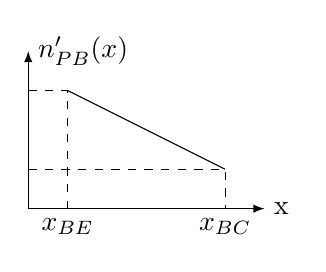
\begin{tikzpicture}
        %asse x
            \draw[-latex](0,0)--++(3,0)node[right]{x};
             %asse y
            \draw[-latex](0,0)--++(0,2)node[right]{$n_{PB}'(x)$};
            %disegno grafico
            \draw(0.5,1.5)--(2.5,0.5);
            %tratteggi
            \draw[dashed](0,1.5)--(0.5,1.5)--(0.5,0)node[below]{$x_{BE}$};
            \draw[dashed](0,0.5)--(2.5,0.5)--(2.5,0)node[below]{$x_{BC}$};
        \end{tikzpicture}
    \end{center}
\end{minipage}
%
\vspace{3mm}\\
%
Io ricordo che la derivata di una retta da come risultato il coefficente angolare. Quindi calcolo il coefficiente angolare della retta che passa tra due punti $X_{BC} $ ed $X_{BE}$ e trovo che:
\begin{align}
   \dfrac{dn'}{dx}&=\dfrac{ n'(x_{BC})-n'(x_{BE})}{W_B} \\
   \dfrac{dn'}{dx} &= \dfrac{n_i^2}{N_{AB}W_B} \left[ e^{\frac{V_{BE}}{V_T}} - 1 \right] -\dfrac{n_i^2}{N_{AB}W_B}\left[] e^{\frac{V_{BC}}{V_T}} - 1 \right]\\
\end{align}

Ora posso calcolare la corrente di diffusione degli elettroni $I_{n,D}$ tramite la formula:

\begin{align}
    I_{n,D}&=qAD_n \dfrac{dn'}{dx}\\
    I_{n,D}(x_{BC})&=+q \dfrac{AD_n n_i^2}{N_{AB} W_B} \left[ e^{\frac{V_{BC}}{V_T}}-1\right] -q \dfrac{AD_n n_i^2}{N_{AB} W_B} \left[ e^{\frac{V_{BE}}{V_T}}-1\right] 
\end{align}
\begin{ricevimento}
    perchè c'è il pedice xbc?? $I_{n,D}(x_{BC})$. non sarebve stato uguale anche in Xbe??
\end{ricevimento}
%
importante:
%
\begin{equation}
    I_{n,D}(x_{BC})=-I_{n,D}(x_{BE})
\end{equation}
%
\begin{exbox}[Metodo del Ghione pg 548]
Per trovare le equazioni delle correnti di diffusione di elettroni devo considerare la distribuzione dei portatori minoritari iniettati dall'emettitore verso la base (la base è drogata p, stò parlando di elettroni).\\
Per questo devo scrivere l'equazione di diffusione per i portatori minoritari in eccesso nella base:
\begin{equation}
    \dfrac{d^2n'}{dx^2}=\dfrac{n'}{L_{nB}^2}
\end{equation}
    partendo da
    %
    \begin{equation*}
        \dfrac{d^2n'}{dx^2}=\dfrac{n'}{L_{nB}^2}
    \end{equation*}
    %
    scrivo la soluzione esprimendola in termini di seni e coseni iperbolici:
    %
    \begin{equation*}
        n'(x)=n'(x_{BE})\dfrac{\sinh{\left( \dfrac{x_{BC}-x}{L_{nB}}\right)}}{\sinh{\left( \dfrac{x_{BC}-x_{BE}}{L_{nB}}\right)}}+ n'(x_{BC})\dfrac{\sinh{\left(\dfrac{x-x_{BE}}{L_{nB}}\right)}}{\sinh{\left( \dfrac{x_{BC}-x_{BE}}{L_{nB}}\right)}}
    \end{equation*}
    %
    Tenendo presente che $ W'_B= x_{BC} — x_{BE}$ è la lunghezza efficace della base (in zona attiva diretta lo spessore della regione di svuotamento dal lato di emettitore è trascurabile, perché la giunzione è polarizzata direttamente, mentre può non esserlo quello della regione di svuotamento dal lato della g1unz1one base-collettore, polarizzata inversamente), e che si approssimerà $W'_B \approx W_B$, si può scrivere: 
    %
    \begin{equation*}
         n'(x)=n'(x_{BE})\dfrac{\sinh{\left( \dfrac{x_{BC}-x}{L_{nB}}\right)}}{\sinh{\left( \dfrac{W_B}{L_{nB}}\right)}}+ n'(x_{BC})\dfrac{\sinh{\left(\dfrac{x-x_{BE}}{L_{nB}}\right)}}{\sinh{\left( \dfrac{W_B}{L_{nB}}\right)}}
    \end{equation*}
    %
    Tenendo presente le equazioni di shotkley e la formula per calcolare $I_{n,D}(x_{BE})$ ed $I_{n,D}(x_{BC})$:
    %
    \begin{alignat*}{2}
        I_{n,D}(x_BE)&=-\dfrac{qAD_n n_i^2}{N_{AB}L_{NB}}\coth{\left( \dfrac{W_B}{L_{nB}}\right)}\left[ e^{V_{BE}/V_T}-1\right]+\dfrac{qAD_n n_i^2}{N_{AB}L_{NB}}\left[\sinh{\left( \dfrac{W_B}{L_{nB}}\right)}\right]^{-1}\left[ e^{V_{BE}/V_T}-1\right] \\
        I_{n,D}(x_BC)&=-\dfrac{qAD_n n_i^2}{N_{AB}L_{NB}}\left[\sinh{\left( \dfrac{W_B}{L_{nB}}\right)}\right]^{-1}\left[ e^{V_{BE}/V_T}-1\right]+\dfrac{qAD_n n_i^2}{N_{AB}L_{NB}}\coth{\left( \dfrac{W_B}{L_{nB}}\right)}\left[ e^{V_{BE}/V_T}-1\right]
    \end{alignat*}
    %
    unisco tutto quello visto precedentemente per calcolare le correnti finali:
    %
    
    \begin{alignat*}{2}
        I_E = &-q \dfrac{AD_p n_i^2}{N_{DE} W_E} \left[ e^{\frac{V_{BE}}{V_T}}-1\right] -q\dfrac{AD_n n_i^2}{N_{AB} W_B}\coth{\left(\dfrac{W_B}{L_{nB}}\right)} \left[ e^{\frac{V_{BE}}{V_T}}-1\right]\\ &+q \dfrac{AD_n n_i^2}{N_{AB} L_{nB}} \left[\sin{\dfrac{W_B}{L_{nB}}}\right]^{-1}\left[ e^{\frac{V_{BE}}{V_T}}-1\right]
        \\
        I_C = &+q \dfrac{AD_n n_i^2}{N_{AB} L_{nB}}\left[\sinh{\left( \dfrac{W_B}{L_{nB}}\right)}\right]^{-1} \left[ e^{\frac{V_{BE}}{V_T}}-1\right] -q\dfrac{AD_p n_i^2}{N_{DC} L_{pC}} \left[ e^{\frac{V_{BC}}{V_T}}-1\right]\\ & -q \dfrac{A D_n n_i^2}{N_{AB} L_{nB}}\coth{\left(\dfrac{W_B}{L_{nB}}\right)} \left[ e^{\frac{V_{BC}}{V_T}}-1\right]
    \end{alignat*}
    %
    Ora considero il caso di base molto corta, al punto che posso approssimare le funzioni iperboliche fino al primo ordine:
    %
    \begin{align*}
        &\coth\left(\dfrac{w_B}{L_{nB}}\right) \approx \dfrac{L_{nB}}{W_B} \\
        &\sinh\left(\dfrac{w_B}{L_{nB}}\right) \approx \dfrac{W_B}{L_{nB}}
    \end{align*}
    %
\end{exbox}
%
\cleardoublepage
Alla fine della fiera troverò le seguenti equazioni:
%
\begin{alignat}{2}
    I_E &= -q \dfrac{AD_p n_i^2}{N_{DE} W_E} \left[ e^{\frac{V_{BE}}{V_T}}-1\right] -q\dfrac{AD_n n_i^2}{N_{AB} W_B} \left[ e^{\frac{V_{BE}}{V_T}}-1\right]  +q \dfrac{AD_n n_i^2}{N_{AB} W_B} \left[ e^{\frac{V_{BC}}{V_T}}-1\right] \label{eq:Ebers-Mole}
    \\
    I_C &= +q \dfrac{AD_n n_i^2}{N_{AB} W_B} \left[ e^{\frac{V_{BE}}{V_T}}-1\right]  \underbrace{-q\dfrac{AD_n n_i^2}{N_{AB} W_B} \left[ e^{\frac{V_{BC}}{V_T}}-1\right]  +q \dfrac{AD_p n_i^2}{N_{DC} W_C} \left[ e^{\frac{V_{BC}}{V_T}}-1\right] }_{(1+\beta)I_{CB0}}
\end{alignat}
se considero i verso in modo tale che $I_B=-I_E-I_C$ avro:
\begin{align}
    I_B &= +q \dfrac{AD_b n_i^2}{N_{DE} W_E} \left[ e^{\frac{V_{BE}}{V_T}}-1\right] +q \dfrac{AD_h n_i^2}{N_{DC} W_C} \left[ e^{\frac{V_{BC}}{V_T}}-1\right] 
\end{align}
Queste sono chiamate \textbf{equazioni di Ebers-Mole}.Posso identificare diverse componenti:
\begin{enumerate}
    \item La corrente di lacune iniettate dalla base nell'emettitore
        \begin{equation}
        +q \dfrac{AD_h n_i^2}{N_{DE} W_E} \left[ e^{\frac{V_{BE}}{V_T}}-1\right]
        \end{equation}
    \item La corrente di lacune iniettate dalla base nel collettore, trascurabile in zona attiva diretta(è la corrente inversa di saturazione)
        \begin{equation}
        +q \dfrac{AD_h n_i^2}{N_{AB} L_{hC}} \left[ e^{\frac{V_{BC}}{V_T}}-1\right]
        \end{equation}
    \item le alre correnti non si sono considerate ma sono a pg 549
\end{enumerate}
Se considero di avere il BJT in RAD $\left( \frac{B_{BC}}{V_T}\ll 1,\frac{B_{BE}}{V_T}\gg 1 \right)$ le componenti con andamento $e^{\frac{V_{BC}}{V_T}}$ diventano trascurabili, permettendomi di approssimare:
\begin{align}
    I_C &\approx I_0 e^{\dfrac{V_{BE}}{V_T}}\\
    I_B &\approx I_S e^{\dfrac{V_{BE}}{V_T}}
\end{align}
e quindi
\begin{align}
    \dfrac{I_C}{I_B}=\beta&=\dfrac{D_n n_{iB}^2}{N_{AB}W_B} \cdot \dfrac{N_{DE}W_E}{D_P n_{iE}^2}
\end{align}
    Se considero l'ipotesi di concentrazione di elettroni intrinseci nel lato base uguali alla concentrazione di elettroni intrinseci nel lato emettitore ($n_{iB}=n_{iE}$):
    \begin{align}
    \beta&=\dfrac{D_n}{D_p} \cdot \dfrac{N_{DE}W_E}{N_{AB} W_B}
\end{align}

Io devo ricordarmi che Il guadagno di un transistor NPN è maggiore di quello di un PNP perchè $D_n>D_h$. Inoltre per avere un elevato guadagno si deve avere il drogaggio della base minore di quello dell'emettitore  ($N_{AB} \ll N_{DE}$) e la lunghezza di base piccola ($W_B \ll W_E$)ma questo non è semplice perchè andrà in conflitto con alcune delle successive osservazioni:

\begin{enumerate}
    \item la base deve essere sottile in modo che la regione neutra della base sia molto sottile
    \item la base, se possibile, deve essere poco drogata.
    \item non posso prender we largo quanto mi pare perchè l'ipotesi di $W_E \ll L_{E}$ non varrebbe più 
    \item Non posso aumentare a dismisura il drogaggio $N_{DE}$ altrimenti diminuisce la mobilità, aumenta la resistività e di conseguenza aumenta al retroazione negativa, perchè si ha una R più grande all'uscita dell'emettitore
    \item meglio avere un BJT npn di un pnp perchè ho $\frac{D_n}{D_h}$, siccome le lacune diffondono meno degli elettroni.
\end{enumerate}
Considerazioni sul comportamento reale della corrente di collettore vengono fatti nella sezione "Elementi di non idealità, effetto Early".\\
%
\subsection{Breakdown del transistor}
Tale sezione è inserita per mantenere il senso logico del discorso che ci sarà successivamente ma non è stato spiegato dal professore.\\
\begin{figure}[hbt!]
    \centering
    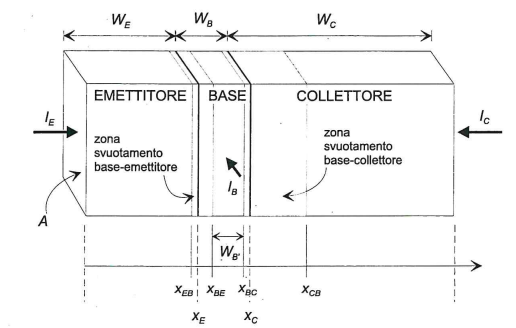
\includegraphics[width=0.5\textwidth]{Immagini_Micro&Nano/Imm_3_Transistor_BJT/npn monodimensionale.png}
    \caption{Caption}%
    \label{fig:enter-label}
\end{figure}\\
La giunzione base collettore influisce debolmente sulla corrente di collettore attraverso l'effetto Early  ma la cosa più importante è che stabilisce la tensione di breakdown del transistore in regione attiva diretta.\\
Il collettore è caratterizzato da una lunghezza $W_C$ e dal drogaggio $N_{DC}$ (in un transistore npn). La lughezza $W_C$ non  influenza le caratteristiche del BJT in regione attiva diretta e normalmente è più lungo rispetto alla base ed all'emettitore per necessità tecnologiche. 
Il motivo dietro la prima affermazione si spiega dal fatto che il collettore ha come unico scopo quello di raccoglie elettroni (portatori maggioritari) provenienti dalla base, e questo processo non involve la lunghezza del collettore (in realtà SI, ma in modo estremamanete trascurabile). Inoltre, la lunghezza del collettore viene presa grande perchè influisce sulle prestazioni del transistor al di fuori della RAD, come velocità di commutazione e guadagno di corrente.\\
Il drogaggio del collettore ha influenza sulle proprietà di breakdown del transistor . La giunzione base-collettore, polarizzata inversamente, presenta due meccanismi di breakdown, la perforazione diretta e il breakdown a valanga.
\subsubsection{Breakdown del BJT: perforazione diretta}
La perforazione diretta è causata dal fatto che la regione di svuotamento della giunzione B-C si allarga al crescere della polarizzazione inversa, ossia di $|V_{BC}|$, fino a raggiungere il punto di rottura.\\
Prima di continuare definisco alcuni parametri:
$\xi_B = x_C-x_{BC}$ è la profondità della regione di svuotamento della giunzione $B_C$ dal lato della base.\\
$\xi_C = x_{CB}-x_{C}$ è la profondità della regione di svuotamento della giunzione $B_C$ dal lato del collettore.\\
Ti ricordi i doscorsi fatti con la regione pn? aumentando la tensione inversa la regione di svuotamento aumenta in maniera proporzionale fino a quando non si ha perforazione, il BJT è uguale:
La perforazione diretta avviene quando $\xi_B \approx W_B$,

ossia quando la regione di svuotamento della regione B-C sì estende sull'intera base (si è trascurato lo spessore della regione E-B dal alto della base). \\
Per base e collettore drogati uniformemente sì ha:
\begin{align}
    \xi_C=\sqrt{\dfrac{2\varepsilon N_{eq}(V_{bi}-V_{BC})}{qN_{DC}^2}}\nonumber\\
    \xi_B=\sqrt{\dfrac{2\varepsilon N_{eq}(V_{bi}-V_{BC})}{qN_{AB}^2}} \nonumber
\end{align}
Dove $\frac{1}{N_{eq}}=\frac{1}{N_{DC}}+\frac{1}{N_{AB}}$ e $V_{bi}$ è la tensione di built-in.\\
Facendo il rapporto dei due si arriva alla formula:
\begin{equation}
    \dfrac{\xi_B}{\xi_C}=\dfrac{N_{DC}}{N_{AB}}
\end{equation}
Poichè la base è molto più sottile del collettore, è necessario fare in modo che il rapporto $\xi_B \ll \xi_C$ sia anch'esso piccolo in modo da evitare la perforazione ($\xi_B \approx W_B$) ossia, per mantenere il campo elettrico nella base basso e prevenire che i portatori di carica assumino  energia in base sufficiente alla perforazione. \\Questa situazione si può ottenere aumentando il drogaggio della base rispetto a quella del collettore:  
\begin{equation}
    N_{AB} \gg N_{DC}
\end{equation}
in definitiva, in un transistor bipolare il drogaggio deve decrescere dall'emettitore alla base al collettore. In queste condizioni $\xi_B=\sqrt{\frac{2\varepsilon N_{DC}(V_{bi}-V_{BC})}{qN_{AB}^2}}$ diventa trascurabile al punto tale da poter approssimare la regione di svuotamento B-C come se fosse data dalla sola $\xi_C=\sqrt{\frac{2\varepsilon N_{DC}(V_{bi}-V_{BC})}{qN_{DC}^2}}$.\\
\subsubsection{Breakdown del BJT: effetto valanga}
Il breakdown a valanga può avvenire in corrispondenza della giunzione base-collettore per polarizzazioni inverse elevate cioè per tensioni  $|V_{BC}|$ oltre la quale il campo elettrico $\mathcal{E}=\sqrt{\dfrac{2qN_{DC}(V_{bi}-V_{BC})}{\varepsilon}}$ raggiunge il valore di soglia per l'innesco della moltiplicazione a valanga. Per rendere minimo $\mathcal{E}$ sì può diminuire il drogaggio del collettore $N_{DC}$. ma è importante sapere che valori troppo bassi di $N_{DC}$ non sono opportuni perché aumentano la resistenza parassita del collettore.  



\section{26.10.2023}
\subsection{Elementi di non idealità}
Il primo elemento di non idealità è che $V_{CE}=V_{CB}+V_{BE}$
\begin{figure}[hbt!]
    \centering
    \begin{circuitikz}
        \draw(0,0)node[left]{B}--++(0.5,0) node[npn,anchor=B](npn){};
        \draw(npn.C)--++(0,0.5)node[above]{C};
        \draw(npn.E)--++(0,-0.5)node[below]{E};
        %Vbc
        \draw[red,-latex] (0.95,0.85) arc (90:180:0.75)node[above]{$V_{BC}$};
        \draw[red,-latex] (0.95,-0.85) arc (270:180:0.75)node[below]{$V_{BE}$};
        \draw[red,-latex] (1.45,-0.5) arc (270:360+90:0.5)node[above]{$V_{BC}$};
    \end{circuitikz}
    \caption{Caption}
    \label{fig:enter-label}
\end{figure}
%
\begin{ricevimento}
    sistemare
\end{ricevimento}

Se $V_{CE}$ aumenta e $VBE \approx V_{th}$, per fare in modo che il dispositivo rimanga attivo (E-B on) e continui ad erogare corrente, $V_{CB}$ dovrà aumentare (ovvero $V_{BC}$ dovrà diventare sempre più negativo), polarizzando maggiormente la B-C in maniera inversa ed aumentando la regione di svuotamento. Per questo motivo la caratteristica tensione corrente nella configurazione emettitore comune ha la seguente forma:
\begin{figure}[hbt!]
    \centering
    
\includegraphics[width=0.15\textwidth,angle=90]{ImmaginiImmagini_Micro&Nano/Imm_3_Transistor_BJT/caratteristicaBJTRAD.png}
    \caption{Caption}%
    \label{fig:enter-label}
\end{figure}

finchè la $V_{CE}$ è bassa, la tensione $V_{BC}$ può essere positiva, così che abbiamo 2 giunzioni polarizzate che mandano la $I_{tot}$ a zero, perchè le due correnti di giunzione idealmente si cancellano.\\
Quando non vi è più compensazione, il diodo non eragà più corrente ma la raccoglie in modo che Itot=cost..
corrente totale dipende solo da Vbe.\\
Si avrà un valore di Ib(Vbe). la tensione chemanda sottosoglia la giunzione BC risulta uguale a circa 0.3V in quanto se $Vce \approx0.2V$ (con $V_{BE}\approx V_{th}$) allora $V_{BC}=0.3V $.\\
la corrente di base aumenta in quanto si ha una riduzione delle ricombinazioni
 
\subsubsection{Effetto Early}

In un primo momento ho considerato il transistor come fosse un componente ideale. Con tale approssimazione ho ottenuto che la corrente  di uscita in RAD ($I_C=I_B/\beta$) è costante al variare della tensione $V_{CE}$ e quindi che il BJT si comporti come un generatore ideale di corrente pilotato dalla sola $I_B$.
Nella realtà  tuttavia, i BJT che operano in RAD hanno una corrente $I_C$ dipendente dalla tensione di uscita ($V_{BC}$ o $V_{CE}$) poichè queste ultime influenzano le dimensioni delle regioni di svuotamento, le quali modificano le correnti.\\

\begin{figure}[hbt!]
    \centering
    \begin{tikzpicture}
        \draw(0,0)--++(12,0);
         %disegno Xe
        \draw[densely dashed](4,0)--++(0,3);
        \draw[>=latex, <-,blue] (4,-0.1)--++(0,-0.5) node [anchor=north,blue]{$x_E$};
         %disegno Xbe
        \draw[densely dashed](4.5,0)--++(0,3);
        \draw[>=latex, <-,blue] (4.5,-0.1)--++(0,-0.3) node [anchor=north,blue]{$x_{BE}$};
         %disegno Xbc
        \draw[densely dashed](8.5,0)--++(0,3);
        \draw[>=latex, <-,blue] (8.5,-0.1)--++(0,-0.3) node [anchor=north,blue]{$x_{BC}$};
        \draw[>=latex, <-,blue] (7.5,-0.1)--++(0,-0.2) node [anchor=north,blue]{$x_{BC}'$};
         %disegno Xc
        \draw[densely dashed](9.5,0)--++(0,3);
        \draw[>=latex, <-,blue] (9.5,-0.1)--++(0,-0.5) node [anchor=north,blue]{$x_{C}$};
        
        \draw[dashed](0,0.5)--++(4,0);
        \draw[dashed](4,0.5)--++(4,0);
        \draw[dashed](8,0.5)--++(4,0)node[right]{$n_i^2$};
        
        \node at (2,3.5)[]{N};
        \node at (6,3.5)[]{P};
        \node at (10,3.5)[]{N};
        \node at (5.5,1.25)[]{$Q_B$};

        \draw[|-|](4.5,-2+0.5)--(8.5,-2+0.5);
        \draw(4.5+2,-1.8)node[]{$W_B$};
        
        \draw[|-|](4.5,-1)--(7.5,-1);
        \draw(4.5+1.5,-0.8)node[]{$W_B'$};
        %grafico rosso    
        \draw[very thick,red] (4.5,2.5)node[right,black]{$n_0$}-- (8.5,0.5);

        %carica
         \draw[pattern=north east lines, pattern color = red] (4.5,0.5)--(4.5,2.5)--(7.5,0.5)--(4.5,0.5);
               
    \end{tikzpicture}
    \caption{Caption}
    \label{fig:enter-label}
\end{figure}
%
Nel caso ideale le regioni di svuotamento sono state sempre di dimensione fissa e quindi anche la base ha sempre avuto larghezza costante $W_B$ indipendentemente dalle tensioni applicate.\\
In realtà lo spessore della base dipende, in regione attiva diretta, dalla tensione applicata alla base perchè al crescere della tensione di polarizzazione (all'aumentare di $V_{CE}$ si modifica $V_{Cb}$ quindi:) la base si assottiglia ($W_B' =W_B- \xi(V_{BC}) \ll W_B$) causando due effetti:
\begin{enumerate}
    \item La corrente emettitore (collettore) aumenta perchè si ha un eccesso della concentrazione dei portatori minoritari base. Graficamente questo corrisponde ad una pendenza della retta maggiore(vedere figura sopra).
\begin{exbox}
    nell'equazione che descrive $I_C$ c'è una dipendenza con Wb/Lnb nella spiegazione del Ghione, prima dell'eq (\ref{eq:Ebers-Mole})
    \begin{center}
        
\includegraphics[width=0.5\textwidth]{Immagini/imm23.10.2023/effetto Early.png}
    \end{center}
\end{exbox}
    Poichè la base è più drogata del collettore la variazione della $W_B$ dovuta alla $V_{BC}$ è resa minima, ma non annullata. Rendere minima questa variazione è una ulteriore ragione per drogare la base più del collettore. 
    \item La corrente di base\_diminuisce perché, diminuendo lo spessore della base, diminuisce  la ricombinazione dei portatori iniettati dall'emettitore con portatori maggioritari nella base. In altri termini, all'aumentare della polarizzazione inversa base-collettore diminuisce il tempo di transito e aumenta $\beta$. Pertanto, se si mantiene costante la corrente di base, la corrente di collettore aumenta ulteriormente.  \\
\end{enumerate}
%
\cleardoublepage
Il punto numero 2 si può studiare in pochi passaggi:\\
%
\begin{minipage}{0.45\textwidth}
    Parto dalla figura dei portatori minoritari all'interno della base comprese le regioni di svuotamento , poi ne considero l'approssimazione lineare.
    
    Il tempo si transito si può calcolare a aprtire di $Q_B$.
    La carica $Q_B$ è l'integrale della distribuzione di carica presenza nella giunzione di base (che abbiamo approssimato come lineare)
    %
    \begin{equation}
        \tau_t=\dfrac{Q}{I_C}
    \end{equation}
    %
    \begin{align}
        I_C &\approx D_n \dfrac{n_0}{W_B}\\
        Q_B&=\dfrac{n_0 W_B}{2}\\
        \tau_t&=\dfrac{1}{2} \dfrac{W_B^2}{D_n}
    \end{align}
    %
\end{minipage}
\hfill%
\begin{minipage}{0.45\textwidth}
    \begin{tikzpicture}[scale=0.65]
        \draw(0,0)--++(12,0);
         %disegno Xe
        \draw[densely dashed](4,0)--++(0,3);
        
         %disegno Xbe
        \draw[densely dashed](4.5,0)--++(0,3);
        
         %disegno Xbc
        \draw[densely dashed](8.5,0)--++(0,3);
        
         %disegno Xc
        \draw[densely dashed](9.5,0)--++(0,3);
       
        
        \draw[dashed](0,0.5)--++(4,0);
        \draw[dashed](4,0.5)--++(4,0);
        \draw[dashed](8,0.5)--++(4,0);

        \node at (2,3.5)[]{N};
        \node at (6,3.5)[]{P};
        \node at (10,3.5)[]{N};

        %grafico rosso
        \draw[very thick,red] (4,2.5) to [out=240,in=1] (0,0.55) ;
        \draw[very thick,red] (4.5,2.5).. controls (5.5,1.5) and (6.2,1.55) .. (6.5,1.45);
        \draw[very thick,red] (6.5,1.45) to [out=-5,in=120] (8.5,0) ;
        \draw[very thick,red] (9.5,0) to [out=20,in=180] (12,0.45) ;

        %tratteggi

        % grafico carica
         \draw[pattern=north east lines, pattern color = gray] (4.5,0)--(4.5,2.5).. controls (5.5,1.5) and (6.2,1.55) .. (6.5,1.45)to [out=-5,in=120] (8.5,0)--(4.5,0);

          \begin{scope}[shift={(0,-4)}]
          
            \draw(0,0)--++(12,0);
             %disegno Xe
            \draw[densely dashed](4,0)--++(0,3);
            \draw[>=latex, <-,blue] (4,-0.1)--++(0,-0.5) node [anchor=north,blue]{$x_E$};
             %disegno Xbe
            \draw[densely dashed](4.5,0)--++(0,3);
            \draw[>=latex, <-,blue] (4.5,-0.1)--++(0,-0.3) node [anchor=north,blue]{$x_{BE}$};
             %disegno Xbc
            \draw[densely dashed](8.5,0)--++(0,3);
            \draw[>=latex, <-,blue] (8.5,-0.1)--++(0,-0.3) node [anchor=north,blue]{$x_{BC}$};
            \draw[>=latex, <-,blue] (7.5,-0.1)--++(0,-0.2) node [anchor=north,blue]{$x_{BC}'$};
             %disegno Xc
            \draw[densely dashed](9.5,0)--++(0,3);
            \draw[>=latex, <-,blue] (9.5,-0.1)--++(0,-0.5) node [anchor=north,blue]{$x_{C}$};
            
            \draw[dashed](0,0.5)--++(4,0);
            \draw[dashed](4,0.5)--++(4,0);
            \draw[dashed](8,0.5)--++(4,0)node[right]{$n_i^2$};
            
            \node at (5.5,1.25)[]{$Q_B$};
    
            \draw[|-|](4.5,-2)--(8.5,-2);
            \draw(4.5+2,-1.8-0.5)node[]{$W_B$};
            
            \draw[|-|](4.5,-1-0.5)--(7.5,-1-0.5);
            \draw(4.5+1.5,-0.8-0.3)node[]{$W_B'$};
            %grafico rosso    
            \draw[very thick,red] (4.5,2.5)node[right,black]{$n_0$}-- (8.5,0.5);
    
            %carica
             \draw[pattern=north east lines, pattern color = red] (4.5,0.5)--(4.5,2.5)--(7.5,0.5)--(4.5,0.5);
          \end{scope}
    \end{tikzpicture}
\end{minipage}
\vspace{3mm}
%
Si capisce quindi che il tempo di transito diminuisce in modo proporzionale al quadrato di $W_B$ e ,dato che $\beta = \frac{\tau_0}{\tau_t}$ , si avrà un aumento del guadagno.\\
%
Se guardo il transistor dal punto di vista del collettore a modo comune:
\begin{center}
    
\includegraphics[width=0.15\textwidth,angle=90]{Immagini/imm23.10.2023/circuitoEarly.jpg}
\end{center}
Senza la $r_{ce}$, colui che produce il suddetto effetto early, si avrebbe un generatore di corrente perfetto
La pendenza implica l'esistenza della reisstenza, che vale in regime dinamico e NOn statico.
\subsubsection{Effetti di basso ed alto livello di iniezione, il diagramma di Gummel}
\begin{exbox}
    Gli effetti dovuti agli alti livelli di iniezioni si studieranno alla fine del corso. anche se non farà parte dell'argomento BJT, la teoria fisica è la stessa.
\end{exbox}
Per spiegare questa non idealità si fà ricorso al diagramma di Gummel. Sì tratta di un grafico in scala semilogaritmica della corrente di collettore e della corrente di base, in funzione della tensione $V_{BE}$, per valori tali da polarizzare direttamente la giunzione base-emettitore, e per un valore costante della tensione $V_{BC}$ tale da polarizzare inversamente la giunzione base-collettore.  Il valore di  $V_{BC}$ è poco importante, a meno che il transistore non presenti un effetto Early anormalmente elevato. 
\begin{figure}[hbt!]
    \centering
    
\includegraphics[width=0.5\textwidth]{Immagini/imm23.10.2023/gummel ideale.png}
    \caption{Caption}
    \label{fig:enter-label}
\end{figure}
Poiché in zona attiva diretta la dipendenza della corrente di base $I_B$ dalla tensione $V_{BE}$ segue idealmente la legge della giunzione pn ($I_B \approx I_0 \cdot \left[e^{V_{BE}/V_T}-1 \right]$), in scala semilogaritmica la curva $I_B(V_{BE})$ è approssimativamente una retta
Ma in regione attiva diretta $I_C \approx \beta I_B$, per cui anche $I_C(V_{BE})$ è una retta in scala semilogaritmica, spostata verso l'alto di $\log_{10}(\beta)$. Un esempio di Gummel plot ricavato dal modello ideale (teoria di Shockley) è mostrato nella figura sopra.\\

In un dispositivo ideale l'amplificazione $\beta$ in regione attiva diretta si mantiene costante per qualsiasi valore di corrente $I_B$ e $I_C$ (basse o alte che siano). Questo non avviene in pratica: in un transistore reale $\beta$ ha un massimo in un campo intermedio di tensioni ma decresce per bassa tensione (basse correnti) e per alte tensioni (alte correnti), come mostrato in Figura:
\begin{figure}[bht!]
    \centering
    
\includegraphics[width=0.5\textwidth]{Immagini/imm23.10.2023/andamento di beta.png}
    \caption{Caption}
    \label{fig:enter-label}
\end{figure}
Il vero diagramma di gummel per un transistore reale risulta essere:
\begin{figure}[hbt!]
    \centering
    
\includegraphics[width=0.5\textwidth]{Immagini/imm23.10.2023/diagramma di gummel.png}
    \caption{Caption}
    \label{fig:enter-label}
\end{figure}

Il diverso comportamento è da attribuirsi alle seguenti cause:  
\begin{enumerate}
    \item Per bassa $V_{BE}$ (e quindi per bassi valori di $I_C$) la corrente di collettore si comporta come $exp(V_{BE}/\eta V_T)$ con fattore di idealità 1 unitario, ma la corrente  di base si comporta come $exp(V_{BE}/\eta V_T)$ con fattore di idealità $\eta >1$, come evidenziato dalla pendenza costante ma inferiore. Il diverso fattore di idealità (di solito prossimo a 2) per la corrente di base è attribuibile, analogamente a quanto visto nel diodo pn, all'effetto della generazione-ricombinazione nelle regioni di carica spaziale. Spesso si ha anche un rilevante effetto di generazione e ricombinazione superficiali. Chiaramente $\eta> 1$ per la corrente di base comporta l'incrocio delle caratteristiche di base e collettore a basse tensioni, ossia il fatto che $\beta$ diviene prima unitario e poi addirittura < 1 per basse tensioni base-emettitore.  
    \item Per alta $V_{BE}$ può divenire significativo l'effetto della resistenza parassita di base, posta in serie all'elettrodo di base intrinseco. Esattamente come accade in un diodo pn polarizzato direttamente, a valori elevati di polarizzazione diretta la tensione applicata cade prevalentemente sulle regioni resistive del diodo. Questo fenomeno giustifica il discostarsi delle caratteristiche dall'andamento rettilineo, ma non la diminuzione di $\beta$.
    \item   Indipendentemente dall'effetto della resistenza parassita di base, per valori elevati di $V_{BE}$ (e quindi per valori elevati di $I_C$) $\beta$ decresce per un insieme di effetti di alta iniezione. ‘Tali effetti sono causati, in una giunzione pn polarizzata direttamente, dal fatto che i portatori minoritari in eccesso iniettati ai due lati della giunzione non sono più trascurabili rispetto ai portatori maggioritari. Anche se i modelli sviluppati sono validi solo in condizioni di basso livello di iniezione, è possibile introdurre in modo qualitativo l'effetto dell'alto livello di iniezione tenendo presente che questo può riguardare sia la base sia il collettore. Si ha allora:  
\begin{enumerate}
    \item     Effetto di alto livello di iniezione nella base: per valori elevati della tensione base-emettitore (transistore npn) la concentrazione degli elettroni  in eccesso iniettati nella base diviene paragonabile con la concentrazione delle lacune maggioritarie nella base. Poiché la base resta, almeno approssimativamente, neutrale, un aumento della concentrazione degli elettroni iniettati oltre il drogaggio della base comporta, per mantenere la neutralità della base, un accumulo di lacune, ossia un aumento del drogaggio equivalente della base. Ma un aumento del drogaggio della base produce una diminuzione dell'efficienza di emettitore, in quanto le lacune in eccesso nella base tenderanno a essere iniettate all'indietro nell'emettitore. Pertanto l'alto livello di iniezione nella base comporta una riduzione dell'amplificazione causata da una ridotta efficienza di emettitore.  
    \item Effetto di alto livello di iniezione nel collettore, detto anche effetto Kirk: come già osservato, ad alta corrente di collettore sì ha forte iniezione di elettroni dall'emettitore alla base (transistore npn), con conseguente richiamo di lacune in eccesso e aumento di drogaggio equivalente nella base. Tale aumento produce un restringimento della regione di carica spaziale base-collettore. Inoltre gli elettroni iniettati nel collettore, che per semplicità si suppone viaggino alla velocità di saturazione nella regione di alto campo base-collettore, schermano parzialmente i donatori ionizzati della regione di carica spaziale tra base e collettore, lato collettore. È quindi come se il drogaggio equivalente del collettore diminuisse. Nel complesso quindi il limite elettrico della base si sposta in avanti verso il collettore, mentre il limite elettrico del collettore neutro si sposta verso il contatto ohmico di collettore (spesso realizzato con un subcollettore $n^+$). L'allargamento della base quasi neutra (base pushout) implica l'aumento del tempo di transito e la diminuzione del $\beta$ del transistore. Per livelli di iniezione estremamente elevata il limite della base oltrepassa $x_C$, ossia il collettore diviene una regione quasi-neutrale con drogaggio trascurabile rispetto alla concentrazione degli elettroni in eccesso iniettati e delle lacune in eccesso che le compensano; in queste condizioni il collettore siì comporta a tutti gli effetti come una regione di tipo p, dando così luogo all'estensione della base fino al limite della regione di subcollettore $n^+$.  
\end{enumerate}
\end{enumerate}
%


\cleardoublepage
\section{BJT: comportamento dinamico}
Vogliamo introdurre un modello matematico del BJT ed un insieme di circuiti equivalenti validi in condizioni di polarizzazione arbitrarie
\subsection{Modello di Ebers-Moll}
Avevo trovato delle espressioni analitiche per le correnti $I_E$ ed $I_C$. Ora le riscrivo nella forma di Ebers-Moll e prenderanno il nome di equazioni di Ebers-Moll pilotate in tensione:
\begin{align}
    I_E&=\mathnormal{a}_{11} \left[ e^{V_{BE}/V_T} -1 \right] +\mathnormal{a}_{12} \left[ e^{V_{BC}/V_T} -1 \right]\\
    I_C&=\mathnormal{a}_{21} \left[ e^{V_{BE}/V_T} -1 \right] +\mathnormal{a}_{22} \left[ e^{V_{BC}/V_T} -1 \right]
\end{align}
Usando queste due equazioni sarò in grado di creare diversi circuiti equivalenti.
\begin{citbox}
    Dove i parametri $\mathnormal{a}_{ij}$[Ampere] assumono una certa equazione solo a assumento transistore a emettitore corto (?), drogaggio uniforme nelle tre regioni e con modello di Shockley. tali equazioni sono:
... pg 574
\end{citbox}

Per motivi spiegati più in dettaglio da Ghione, si avrà che
\begin{itemize}
    \item $a_{12}=a_{21}$
    \item $a_{11} \neq a_{22}$ perchè si considera l'approssimazione di drogaggio del collettore diverso da quello dell'emettitore.
    Sono prese diverse per mitigare il meccanismo che conduce all'effetto Early (riduzione di $W_B$ e conseguente aumento di $I_C$).
    Avremo la seguente situazione:
    \begin{center}
        \includegraphics[width=0.25\textwidth,angle=90]{Immagini/imm26.10.2023/drogaggioBJT.png}
    \end{center}
    Dove $N_{DE}>N_{AB}$ ènecessario per avere $\beta$ alto. $N_{AB}>N_{DC}$ mi garantisce minore variazione di $W_B$ in RAD perchè la regione di svuotamento si estenderà per lo più verso il collettore. Questa scelta, pur ducendo lo svuotamento in base provoca l'aumento della resistività.\\
    Per trovare un compromesso tra bassaresistività e contenimento dell'effetto early si realizza un primo tratto in cui $N_DC<N_{AB}$ e poi un bulck con $N_{DC}^B>N_{AB}$. cioè doppia diffusione .\\
    $\sigma=qN_D\mu_n$ e $\rho=1/\sigma$
\end{itemize}
Per individuare i valori di aij non si usano le formulazioni viste in precedenza, in quanto sperimentalemnte è complesso da studiare le costanti che compongono i parametri aij.
Per fare ciò passo al circuito equivalente di ebers mole.



\begin{citbox}[Come mai vale questa relazione?]
    questo valore non è casuale e vale per ogni transistore reale. Infatti per $V_{BE}\ll V_T, V_{BC}\ll V_T$ il transistore è prossimo all'equilibrio termodinamico ed i termini esponenziali si possono linearizzare, conducendo all'approssimazione:
..
\end{citbox}
\subsubsection{Circuito equivalenti di ebers moll I}
Consideriamo un BJT npn in regione attiva diretta.\\
Ricordo che la corrente $I_C$ (Formula: \ref{eq:formula Ic ebers-moll}) può essere ricavata attraverso la manipolazione matematica del parametro "fattore di trasporto in base ($b$)" ed ha la forma:
\begin{equation}
    I_C=-\alpha_F I_E +I_{CB0}
\end{equation}
dove il pedice F indica la condizione di regione attiva diretta.
Poichè $I_{CB0}$ è la corrente di saurazione inversa della giunzione B-C, si può supporre che per tensioni arbitrarie applicate alla giunzione B-C si possa scrivere
\begin{equation}
    I_C = -\alpha_F I_E +I_{CB0}\left[ e^{V_{BC}/V_T} -1 \right]
\end{equation}
Analoga situazione in regione attiva inversa:

\begin{equation}
    I_E=-\alpha_R I_C +I_{EB0}
\end{equation}
dove $I_{EB0}$ è la corrente di saturazione inversa della giunzione base-emettitore,
polarizzata inversamente in regione attiva inversa. In generale si potrà allora
scrivere: 
\begin{equation}
    I_E = -\alpha_R I_C +I_{EB0}\left[ e^{V_{BE}/V_T} -1 \right]
\end{equation}
Guardando queste equazioni dal punto di vista circuitale, vediamo che richiamano la seconda legge di Khirchoff, la legge dei Nodi, dove $I_{CB0}\left[ e^{V_{BC}/V_T} -1 \right]$ ed $I_{EB0}\left[ e^{V_{BE}/V_T} -1 \right]
$
sono le correnti dei diodi ideali pilotati dalle tensioni $V_{BE}$ e $V_{BC}$ mentre i termini $-\alpha_R I_C$ e $-\alpha_F I_E$ corrispondono a due generatori di corrente pilotati in corrente.\\
Da qui si ottiene il primo circuito equivalente di Ebers-Moll II:
\begin{figure}[hbt!]
    \centering
    \begin{tikzpicture}
        \draw (0,0) node[left]{E}
        to [short,*-]++(1,0)
        to [short]++(0,-0.75)
        to [D,invert]++(2,0)
        to [short]++(0,+0.75)
        to [short]++(1,0) coordinate(b)
        
        (b) to [short,*-*]++(0,-1.5)node[right]{B}
        
        (b) to [short]++(1,0)
        to [short]++(0,0.75)
        to [I, l^=$\alpha I_E$]++(2,0)
        to [short]++(0,-0.75)
        to [short,-*]++(1,0)node[right]{C};
    \end{tikzpicture}
    \caption{Caption}
    \label{fig:enter-label}
\end{figure}
\\%
%Dove le equazioni ai nodi sono:
%\begin{align}
 %   I_E &= \alpha_R I_C +I_{EB0}\left[ e^{V_{BE}/V_T} -1 \right]\\
  %  I_C &= \alpha_F I_E +I_{EB0}\left[ e^{V_{BC}/V_T} -1 \right]
%\end{align}
Sapendo che il BJT tecnologicamente è pressochè simmetrico, a meno di un differente drogaggio, il circuito equivalente finale risulterà essere :
%
\begin{figure}[hbt!]
    \centering
    \begin{tikzpicture}
        \draw (0,0) node[left]{E}
        to [short,*-]++(1,0)
        to [short]++(0,-0.75)
        to [D,invert]++(2,0)
        to [short]++(0,+0.75)
        to [short]++(1,0) coordinate(b)
        
        (b) to [short,*-*]++(0,-1.5)node[below]{B}
        
        (b) to [short]++(1,0)
        to [short]++(0,0.75)
        to [I, l^=$\alpha_F I_E$]++(2,0)
        to [short]++(0,-0.75)
        to [short,-*]++(1,0)node[right]{C};

        \draw (0,0)
        to [short,*-*]++(1,0)
        to [short]++(0,+0.75)
        to [I, l^=$\alpha_R I_C$,invert]++(2,0)
        to [short,-*]++(0,-0.75)
        to (b)
                
        (b) to [short,-*]++(1,0)
        to [short]++(0,-0.75)
        to [D]++(2,0)
        to [short,-*]++(0,+0.75)
        to [short,-*]++(1,0)node[right]{C};

        %labels
        \draw[-latex] (8,-0.25) --++ (-0.75,0)node[midway, below] {$I_C$}; %Ic
        \draw[-latex] (4.25,-1.25) --++ (0,1)node[midway, right] {$I_B$}; %Ib
        \draw[-latex] (0,-0.25) --++ (0.75,0)node[midway, below] {$I_E$}; %Ie

        %corrente diodi
        \draw[-latex] (1.5,-1.25) --++ (+1,0)node[midway, below] {$I_{EB0}\left[e^{{V_{BE}}/{V_T}}-1\right]$}; %Idc

        \draw[-latex] (8-1.5,-1.25) --++ (-1,0)node[midway, below] {$I_{CB0}\left[e^{{V_{BC}}/{V_T}}-1\right]$}; %Idc
        ;
    \end{tikzpicture}
    \caption{Caption}
    \label{fig:enter-label}
\end{figure}
%
\cleardoublepage
\subsubsection{Circuito equivalente di Ebers-Moll II o a iniezione}
Cambiano pilotaggio dei generatori dipendenti, facendo in modo che siano pilotati dalle correnti dei diodi invece dalle correnti di ingresso.\\
riscriviamo le equazioni come:
\begin{align}
    I_E &= -\dfrac{I_{EB0}}{1-\alpha_R \alpha_F}  \cdot \left[ e^{V_{BE}/V_T} -1 \right] 
        +\dfrac{\alpha_R I_{CB0}}{1-\alpha_R \alpha_F} \cdot \left[ e^{V_{BE}/V_T} -1 \right]\\
    I_C &= +\dfrac{\alpha_F I_{EB0}}{1-\alpha_R \alpha_F} \cdot \left[ e^{V_{BC}/V_T} -1 \right]
        -\dfrac{I_{CB0}}{1-\alpha_R \alpha_F}  \cdot \left[ e^{V_{BC}/V_T} -1 \right] 
\end{align}
%
\begin{exbox}
    Precedentemente ho visto come variano le relazioni a connettore comeune tra collettore e VCE:
\end{exbox}
%
Ponendo:
\begin{align}
    \dfrac{I_{EB0}}{1-\alpha_R \alpha_F}  &= I_{E0}\\
    \dfrac{I_{CB0}}{1-\alpha_R \alpha_F}  &= I_{C0}
\end{align}
Si ottiene:
\begin{align}
    I_E &= - I_{E0}  \cdot \left[ e^{V_{BE}/V_T} -1 \right] +\alpha_R I_{C0} \cdot \left[ e^{V_{BE}/V_T} -1 \right]\\
    I_C &=  \alpha_F I_{E0} \cdot \left[ e^{V_{BC}/V_T} -1 \right] -I_{C0}  \cdot \left[ e^{V_{BC}/V_T} -1 \right] 
\end{align}
Dove vale al relazione $\alpha_R I_{C0}=\alpha_F I_{E0}$.\\
Di seguito la realizzazioen circuitale delle precedenti equazioni:
%

\begin{figure}[hbt!]
    \centering
    \begin{tikzpicture}
        \draw (0,0) node[left]{E}
        to [short,*-]++(1,0)
        to [short]++(0,-0.75)
        to [D,invert]++(2,0)
        to [short]++(0,+0.75)
        to [short]++(1,0) coordinate(b)
        
        (b) to [short,*-*]++(0,-1.5)node[below]{B}
        
        (b) to [short]++(1,0)
        to [short]++(0,0.75)
        to [I, l^=$\alpha_F I_{F} $,invert]++(2,0)
        to [short]++(0,-0.75)
        to [short,-*]++(1,0)node[right]{C};

        \draw (0,0)
        to [short,*-*]++(1,0)
        to [short]++(0,+0.75)
        to [I, l^=$\alpha_R I_R$]++(2,0)
        to [short,-*]++(0,-0.75)
        to (b)
                
        (b) to [short,-*]++(1,0)
        to [short]++(0,-0.75)
        to [D]++(2,0)
        to [short,-*]++(0,+0.75)
        to [short,-*]++(1,0)node[right]{C};

        %labels
        \draw[-latex] (8,-0.25) --++ (-0.75,0)node[midway, below] {$I_C$}; %Ic
        \draw[-latex] (4.25,-1.25) --++ (0,1)node[midway, right] {$I_B$}; %Ib
        \draw[-latex] (0,-0.25) --++ (0.75,0)node[midway, below] {$I_E$}; %Ie

        %corrente diodi
        \draw[latex-] (1.25,-1.25) --++ (+1,0)node[midway, below] {$I_F=I_{E0}  \cdot \left[ e^{V_{BE}/V_T} -1 \right]$}; %Idc

        \draw[latex-] (8-1.25,-1.25) --++ (-1,0)node[midway, below] {$I_R=I_{C0}  \cdot \left[ e^{V_{BC}/V_T}-1\right] $}; %Idc
        ;
    \end{tikzpicture}
    \caption{Caption}
    \label{fig:enter-label}
\end{figure}
%
\begin{figure}[hbt!]
    \centering
    \includegraphics[width=0.5\textwidth]{Immagini/imm26.10.2023/circuiti equivalenti ebers moll in tutte le config.png}
    \caption{Caption}
    \label{fig:enter-label}
\end{figure}
%
\begin{figure}[hbt!]
    \centering
    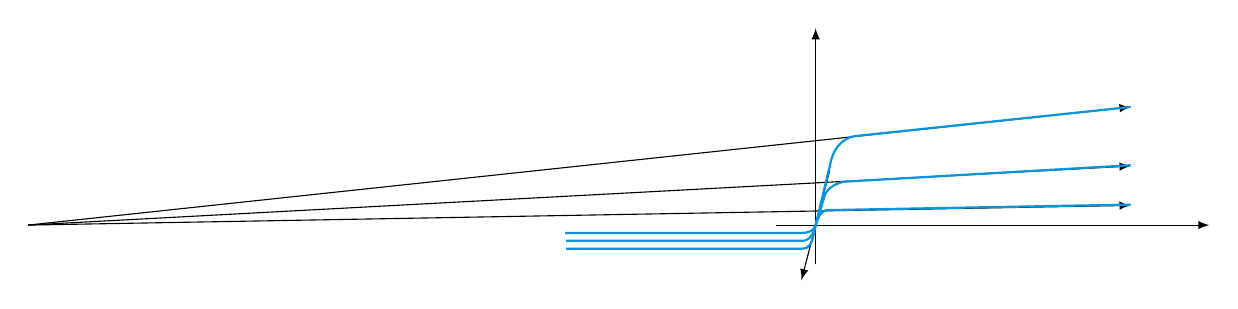
\begin{tikzpicture}[scale=1]
        % asse x
        \draw[-latex](-0.5,0)--(5,0);
        % asse y
        \draw[-latex](0,-0.5)--(0,2.5);
        
        \draw[-latex](-10,0)--(4,0.25);
        \draw[-latex](-10,0)--(4,0.75);
        \draw[-latex](-10,0)--(4,1.5);

        \draw[-latex] (0.18,0.7)--(-0.18,-0.7); 
        %disegno grafico V>0
        \draw[thick,cyan!80!blue](0,0) to [out=70,in=185] (0.15,0.19) -- (4,0.26);
        \draw[thick,cyan!80!blue](0,0)--(0.1,.325 )to [out=80,in=195] (0.35,0.55) -- (4,0.76);
        \draw[thick,cyan!80!blue](0,0)--(0.18,0.75 )to [out=80,in=190] (0.50,1.13) -- (4,1.5);

        %disegno grafico V<0
        \draw[thick,cyan!80!blue](0,0) to [out=255,in=0] (-0.18,-0.1) -- ++(-3,0);
        \draw[thick,cyan!80!blue](0,0) to [out=255,in=0] (-0.17,-0.2) -- ++(-3,0);
        \draw[thick,cyan!80!blue](0,0) to [out=255,in=0] (-0.17,-0.3) -- ++(-3,0);
        %\draw[thick,cyan!80!blue](0,0) to [out=270,in=-185] (-0.15,-0.1) -- ++(-4,0);
        
    \end{tikzpicture}   
    \caption{Caption}
    \label{fig:enter-label}
\end{figure}
%
\subsection{Caratteristiche statiche}
Usando il modello circuitale di Ebers-Moll posso andare studiare le caratteristiche ideali e reali di un BJT (npn).
\subsubsection{Caratteristiche statiche ideali}
FIG\\
\\
QUando entrambe le giunzioni sono polarizzate direttamente ($V_{BC}>|V_{th}|, V_{BE}>V_{th}$) si hanno due correnti opposte che si cancellano. Man mano che la tensione di collettore aumenta, B-C và in OFF, invertendosi, realizzando lo scivolo energetico visto nel diagramma abande.\\
\begin{equation}
    \dfrac{I_B}{I_C}=\beta=\dfrac{\alpha_F}{1-\alpha_F}\approx 100 \ , \text{se }\ \alpha_F=0.99
\end{equation}
Se volessi lavorare in una condizione reverse, il comportamento è analogo ma a causa di $\alpha_R$ molto basso a causa della differenza dei drogaggi
%
\begin{equation}
    \beta^{REV}=\dfrac{D_n}{D_p}\cdot \dfrac{N_{DC}}{N_{AB}}\dfrac{W_C}{W_B} \ \text{con }\ N_{DC}\gg N_{AB}
\end{equation}
%
\subsubsection{Configurazione common base}
Andamento della corrente Ic in uscita in funzione della Ie in ingresso.
FIG\\
\\

\subsubsection{Caratteristiche statiche reali}
La più grande differenza dal mondo ideale è le equazioni di Ebers-Moll non descrivono due effetti dovuti alla non idealità dei componenti: il breakdown e l'effetto Early. Questi verranno spiegati nelle successive sezioni.
\paragraph{Polarizzazione del transistor bipolare}\mbox{}\\
pg587
%
\cleardoublepage 

\subsection{Modello del BJT per piccoli segnali}
In condizioni di piccolo segnale il transistore è eccitato da un generatore tempo-variante (di solito, sinusoidale) di ampiezza “piccola” rispetto alla polarizzazione in continua. In questo caso è possibile dividere le correnti e le tensioni  del
transistore, indicate con lettere minuscole e pedici maiuscoli, in una componente continua, indicata con lettera maiuscola, e in una componente alternata di piccolo segnale, indicata con lettera minuscola: 
\begin{align*}
    i_C(t)&= I_C + i_C(t)\\
    i_E(t)&= I_E + i_E(t)\\
    i_B(t)&= I_B + i_B(t)\\
    v_{BC}(t)&=V_{BC} + v_{BC}(t)\\
    v_{BE}(t)&=V_{BE} + v_{BE}(t)\\
    v_{CE}(t)&=V_{CE} + v_{CE}(t)
\end{align*}

pg 592--usare appunti pieraccini

\subsubsection{Circuito equivalente a $\pi$ di piccolo segnale }
%
Considero un BJT ad emettitore comune.\\
Se voglio rappresentare il circuito equivalente a $\pi$ devo prima calcolare gli elementi della matrice a conduttanze usando le equazioni di $I_E$ , $I_B$ ed $I_C$  statiche ad emettitore comune.
%
\begin{exbox}
    Si parte dalle caratteristiche a base comune (ottenute da ebers Mole II):
    \begin{align}
    I_E &= - I_{E0}  \cdot \left[ e^{V_{BE}/V_T} -1 \right] +\alpha_R I_{C0} \cdot \left[ e^{V_{BE}/V_T} -1 \right]\\
    I_C &=  \alpha_F I_{E0} \cdot \left[ e^{V_{BC}/V_T} -1 \right] -I_{C0}  \cdot \left[ e^{V_{BC}/V_T} -1 \right] 
\end{align}
%
e si pone $I_B=-I_E-I_C$, $V_{BC}=V_{BE}-V_{CE}$. Si ottiene:
%
\begin{align}
    I_B&=(1-\alpha_F)I_{E0}\left( e^{v_{BE}/V_T}-1\right)+(1-\alpha_R)I_{C0}\left(e^{v_{BE}/V_T}e^{-v_{CE}/V_T} -1\right) \\
     I_C&=\alpha_FI_{E0}\left( e^{v_{BE}/V_T}-1\right)-I_{C0}\left(e^{v_{BE}/V_T}e^{-v_{CE}/V_T} -1\right)
\end{align}
\end{exbox}
%
Gli elementi della matrice conduttanza saranno:
%
\begin{align}
    g_{BB} &= \left.\dfrac{di_B}{dv_{BE}}\right|_{V_{BE},V_{CE}}  &  g_{m} &= \left. \dfrac{di_C}{dv_{BE}}\right|_{V_{BE},V_{CE}} \\
    g_{BC} &= \left. \dfrac{di_B}{dv_{BC}}\right|_{V_{BE},V_{CE}}  & g_{CC} &= \left. \dfrac{di_B}{dv_{BC}}\right|_{V_{BE},V_{CE}} \nonumber
\end{align}
%
\begin{figure}[hbt!]
    \centering
    \begin{tikzpicture}
        \draw (0,-2) to [short,*-]++(0.01,0) node[left]{E} coordinate(e);
        \draw(0,0) node[above]{B} 
         to [short,*-*]++(1,0) coordinate(a)
         to [short]++(1.5,0) coordinate (f')
         to [open]++(1.5,0) coordinate (x)
         to [short,-*]++(2,0) coordinate (y)
         to [short,-*]++(1,0)node[above]{C}

         (a) to [R,l=$g_{BB}$,-*]++(0,-2) -| (e) 

         (f') to [I,-*]++(0,-2) node[below]{$g_{BC}$} -| (e) 
         (x) to [I,l=$g_mV_{BE}$,-*]++(0,-2)node[below]{$g_{m}$} -| (e) 
         
         (y) to [R,l=$g_{CC}$,-*]++(0,-2)  to [short,-*]++(1,0) -| (e) 
         ;
         
    \end{tikzpicture}
    \caption{Caption}
    \label{fig:enter-label}
\end{figure}
%
\begin{exbox}
    \begin{align}
    g_{BB} &= \left.\dfrac{di_B}{dv_{BE}}\right|_{V_{BE},V_{CE}} = \dfrac{(1-\alpha_F)I_{E0}}{V_T}e^{V_{BE}/V_T}-\dfrac{(1-\alpha_R)I_{C0}}{V_T}e^{V_{BE}/V_T}e^{-V_{CE}/V_T}\\
    g_{m} &= \left. \dfrac{di_C}{dv_{BE}}\right|_{V_{BE},V_{CE}}=-\dfrac{(1-\alpha_R)I_{C0}}{V_T}e^{V_{BE}/V_T}e^{-V_{CE}/V_T}\\ 
    g_{BC} &= \left. \dfrac{di_B}{dv_{BC}}\right|_{V_{BE},V_{CE}}= \dfrac{\alpha_F I_{E0}}{V_T}e^{V_{BE}/V_T}-\dfrac{\alpha_R I_{C0}}{V_T}e^{V_{BE}/V_T}e^{-V_{CE}/V_T}\\
    g_{CC} &= \left. \dfrac{di_B}{dv_{BC}}\right|_{V_{BE},V_{CE}}= \dfrac{I_{C0}}{V_T}e^{V_{BE}/V_T}e^{-V_{CE}/V_T}\\
\end{align}
Nella condizione di regione attiva diretta si applicano diverse semplificazioni dovute al fatto che $V_{BE}-V_{CE}=V_{BC}<0$. Allora
%
\begin{align}
    i_B &\approx (1-\alpha_F)I_{E0}e^{v_{BE}/V_T}\\
    i_C &\approx \alpha_F I_{E0}e^{v_{BE}/V_T}
\end{align}
%
A seguito di questa approssimazione si avrnno le correnti $i_B$ ed $i_C$ indipendenti alla tensione $v_{CE}$. Di conseguenza si dovrebbe ottenere $g_{BC}= g_{CC} = 0$ ma se voglio modellizzare il comportamento del BJT in modo che sia quanto più possibile fedele alla realtà (sempre sotto certe approssimazioni) dovrò considerare l'incremento della pendenza di $i_C$ dato dall'effetto Early.
Questo incremento di pendenza lo posso tenere in contro dentro i parametri $g_{BC}, g_{CC}$ tenendo presente che:
%
\begin{align}
    \dfrac{\Delta I_C}{\Delta V_{CE}} &\approx \dfrac{I_C}{V_{Early}}\\
    \Delta I_B &\approx -\dfrac{\Delta I_C}{\beta}
\end{align}
%
IMPORTANTE: il segno negativo dipende dal fatto che, mantenendo costante la tensione
base-emettitore, la corrente di base diminuisce a causa dell'effetto Early (perché
diminuisce la carica in eccesso nella base e quindi la ricombinazione nella base).

\begin{ripasso}[da elettronica generale]
    $V_{Early}$ è diverse decine di volt (raggiunge anche il centinaio), $i_B$ è dell'ordine del $\mu A$, $\beta$ è diverse centinaia (tipicamente 300) mentre $i_C$, seppur dipendente dal tipo di applicazione è, di solito, dell'ordine del ($m A$).\\
    Quindi $g_{BC}, g_{CC} \approx 0$ anche se, ripeto, $i_C$ potrebbe essere anche più grande, a seconda dell'applicazione.
\end{ripasso}
%
\end{exbox}
%
Si ottiene, nell'approssimazione di regione attiva diretta ($V_{BE} — V{CE} = V_{BC} < 0$):
%
\begin{equation}
    g_{BB} \approx \dfrac{I_B}{V_T}=\dfrac{I_C}{\beta V_T}
\end{equation}
%
\begin{equation}
    g_{BC} \approx \dfrac{I_B}{V_{Early}} = -\dfrac{I_C}{\beta V_{EARLY}} \approx 0
\end{equation}
%
\begin{equation}
    g_{CB}=g_{m} \approx \dfrac{I_C}{V_T} =\beta \dfrac{I_B}{V_{T}}
\end{equation}
%
\begin{equation}
    g_{CC} \approx \dfrac{I_C}{V_{Early}}
\end{equation}
%
Le equazioni precedenti possono essere utilizzate per definire gli elementi del circuito equivalente a $pi$ nella configurazione a emettitore comune.
Imponendo $|g_{BB}|\gg|g_{BC}|$,$|g_{CB}|\gg|g_{BC}|$,$|g_{CC}|\gg|g_{BC}|$, si avrà che: 
%
\begin{align}
    r_{BE}&=\dfrac{1}{g_{BB}+g_{BC}}\approx \dfrac{1}{g_{BB}}=\dfrac{V_T}{I_B}= \beta \dfrac{V_T}{I_C} \\
    r_{BC}&= \dfrac{1}{-g_{BC}}= \beta \dfrac{V_{Early}}{I_C} \\
    g_m &=g_{CB}-g_{BC}\approx \beta \dfrac{I_B}{V_T} \\
    r_{CE} &= \dfrac{1}{g_{CC}+g_{BC}}\approx \dfrac{1}{g_{CC}}= \dfrac{V_{Early}}{I_C} \\
\end{align}
%
Gli elementi $r_{BC}$ e $r_{CE}$ hanno valore elevato e possono essere spesso sostituiti da circuiti aperti.\\
Spesso il circuito equivalente a $\pi$ può essere modificato per tener
conto della resistenza parassita di base, aggiungendo la resistenza
serie parassita $r_{BB}$ all'incresso della base
%
\begin{figure}[hbt!]
    \centering
    \begin{tikzpicture}
        \draw (0,-2) to [short,*-]++(0.01,0) coordinate(e);
        \draw(0,0) node[above]{B} 
         to [R,l=$r_{BB'}$,*-*]++(2,0) coordinate(a)
         to [R,l=$r_{BC}$,-*]++(2,0) coordinate (x)
         to [short,-*]++(2,0) coordinate (y)
         to [short,-*]++(1,0)node[above]{C}

         (a) to [R,l=$r_{BE}$,-*]++(0,-2) -| (e) 

         (x) to [I,l=$g_mV_{BE}$,-*]++(0,-2) node[below]{E} -| (e) 
         
         (y) to [R,l=$r_{CE}$,-*]++(0,-2) to [short,-*]++(1,0) -| (e) 
         ;
         %label
         \draw[-latex] (-1,0) -- ++(0.75,0) node[midway, above] {$I_B$};
         \draw[latex-] (7.25,0)--++(+1,0) node[midway, above] {$I_C$};
         \draw[-latex] (0,-1.75)--++(0,1.5) node[midway, left] {$V_{BE}$};
         \draw[-latex] (7,-1.75)--++(0,1.5) node[midway, right] {$V_{CE}$};
    \end{tikzpicture}
    \caption{Caption}
    \label{fig:enter-label}
\end{figure}\\
%
Approssimando $r_{BC}$ come circuito aperto e inserendo $r_{BB'}$ dentro $r_{BE}$ si otterrebbe
%
\begin{figure}[hbt!]
    \centering
    \begin{tikzpicture}
        \draw (0,-2) to [short,*-]++(0.01,0) coordinate(e);
        \draw(0,0) node[above]{B} 
         to [short,*-]++(2,0) coordinate(a)
         to [open]++(2,0) coordinate (x)
         to [short,-*]++(2,0) coordinate (y)
         to [short,-*]++(1,0)node[above]{C}

         (a) to [R,l=$r_{BE}$,-*]++(0,-2) -| (e) 

         (x) to [I,l=$g_mV_{BE}$,-*]++(0,-2) node[below]{E} -| (e) 
         
         (y) to [R,l=$r_{CE}$,-*]++(0,-2) to [short,-*]++(1,0) -| (e) 
         ;
         %label
         \draw[-latex] (-1,0) -- ++(0.75,0) node[midway, above] {$I_B$};
         \draw[latex-] (7.25,0)--++(+1,0) node[midway, above] {$I_C$};
         \draw[-latex] (0,-1.75)--++(0,1.5) node[midway, left] {$V_{BE}$};
         \draw[-latex] (7,-1.75)--++(0,1.5) node[midway, right] {$V_{CE}$};
    \end{tikzpicture}
    \caption{Caption}
    \label{fig:enter-label}
\end{figure}
%
\begin{exbox}[perchè mi voglio male]
In un primo momento posso pensare di risolvere usando il teorema di miller, per "disaccoppiare" B e C, collegate da $R_{BC}$.
Definendo $K=\dfrac{V_{CE}}{V_{BE}}$ avrò a sinistra $Z'=\dfrac{Z}{1-K}$ ed a destra avrò $Z''=\dfrac{KZ}{K-1}$.\\
togliendo di mezzo la resistenza parassita di base $r_{BB'}$, avrò:
\begin{align*}
    V_{BE}&=I_B \cdot r_{BE}\\
    V_{CE}&=(I_C-g_mV_{BE})\cdot r_{CE}
\end{align*}
\begin{center}
    \begin{tikzpicture}
        \draw (0,-2) to [short,*-]++(0.01,0) coordinate(e);
        \draw(0,0) node[above]{B} 
         to [R,l=$r_{BB'}$,*-*]++(2,0) coordinate(a)
         to [short]++(1.5,0) coordinate (f')
         to [open]++(2,0) coordinate (f'')
         to [short]++(1.5,0) coordinate (x)
         to [short,-*]++(2,0) coordinate (y)
         to [short,-*]++(1,0)node[above]{C}

         (a) to [R,l=$r_{BE}$,-*]++(0,-2) -| (e) 

         (f') to [generic,l=$Z'$,-*]++(0,-2) -| (e) 
         (f'') to [generic,l=$Z''$,-*]++(0,-2) -| (e) 
         (x) to [I,l=$g_mV_{BE}$,-*]++(0,-2) node[below]{E} -| (e) 
         
         (y) to [R,l=$r_{CE}$,-*]++(0,-2) to [short,-*]++(1,0) -| (e) 
         ;
         %label
         \draw[-latex] (-1,0) -- ++(0.75,0) node[midway, above] {$I_B$};
         \draw[latex-] (7.25+3,0)--++(+1,0) node[midway, above] {$I_C$};
         \draw[-latex] (0,-1.75)--++(0,1.5) node[midway, left] {$V_{BE}$};
         \draw[-latex] (7+3,-1.75)--++(0,1.5) node[midway, right] {$V_{CE}$};
    \end{tikzpicture}
    \captionof{figure}{caption miller pi greco}
    \begin{citbox}
        continuare a risolvere da me
    \end{citbox}
\end{center} 
\end{exbox}


\cleardoublepage
\subsubsection{Comportamento in frequenza}
i modelli precedenti non contengono elementi reattivi anche se a ben pensarci, le giunzioni pn ed np si comportano un anche come delle capacità.
%
\begin{figure}[hbt!]
    \centering
    \begin{tikzpicture}
        \draw (0,-2) to [short,*-]++(0.01,0) coordinate(e);
        \draw(0,0) node[left]{B}
         to [short,*-]++(1,0) coordinate (Cbe)
         to [C,l=$C_{BE}$,*-*]++(0,-2) -| (e)

         (Cbe) to [short,-*]++(2,0) coordinate(a)
         to [R,l=$r_{BC}$,-*]++(2,0) coordinate (x)
         to [short,-*]++(2,0) coordinate (y)
         to [short,-*]++(1,0)node[right]{C}

         (a) to [R,l=$r_{BE}$,-*]++(0,-2) -| (e) 
         
         (a) to [short]++(0,1) 
         to [C,l=$C_{BC}$]++(2,0) to [short,-*]++(0,-1) 

         (x) to [I,l=$g_mv_{BE}$,-*]++(0,-2) node[below]{E} -| (e) 
         
         (y) to [R,l=$r_{CC}$,-*]++(0,-2) to [short,-*]++(1,0) -| (e) 
         ;
    \end{tikzpicture}
    \caption{Caption}
    \label{fig:enter-label}
\end{figure}
%
Le capacità sono trascurabili quando il segnale varia lentamente ma per applicazioni a Radiofrequenza è necessario studiarli perchè  non saranno più approssimabili come circuiti aperti ma avranno impedenza capacitiva molto piccola.\\
è necessario introdurre nel circuito a $\pi$ le capacità di giunzione che sono, in regione attiva diretta:
%
\begin{enumerate}
    \item Capacità B-E $C_{BE}$. Siccome la giunzione B-E è polarizzata direttamente, si tratta in prima approssimazione di una capacità di diffusione legata alla carica in eccesso accumulata nella base. (Se l'efficienza di emettitore è elevata, si può trascurare la componente capacitiva associata alla carica in eccesso iniettata dalla base nell'emettitore.) 
    Il calcolo di questa capacità non ha lo stesso risultato di quello nella giunzione pn perchè nel BJT la base è corta. \\Si può peraltro definire: 
    \begin{align}
        C_{BE} = \dfrac{dQ_B}{dV_{BE}} = \dfrac{dQ_B}{dI_C} \cdot \dfrac{dI_C}{dV_{BE}}
    \end{align}
    ma, tenendo presente la discussione sul tempo di transito in base ($\tau_t=\left|\frac{dQ_B}{dI_E}\right|$) e che \\ $\left|\frac{dI_E}{dV_{BE}}\right| \approx \left|\frac{dI_C}{dV_{BE}}\right| = g_m$, si ha :
    \begin{equation}
    C_{BE}= \textcolor{red}{\tau_t \cdot g_m} =\frac{\tau_t I_C}{V_T}=\frac{\tau_0 I_B}{V_T}
\end{equation}
    dove $\tau_0$ è la vita media dei portatori minoritari nella base, e si è utilizzata la definizione $\beta \approx \frac{\tau_0}{\tau_t}$. 

    \item Capacità base-collettore $C_{BC}$: poiché la relativa giunzione è polarizzata inversamente, si tratta di una capacità della regione di svuotamento (prevalentemente dal lato collettore, meno drogato), di solito molto bassa. 
\end{enumerate}

Il mio obiettivo è determinare la frequenza oltre il quale il dispositivo non è più utilizzabile secondo le specifiche. Infatti, a frequenze elevate le capacità base-emettitore e base-collettore tendono a cortocircuitare le rispettive giunzioni, e l'amplificazione del transistore si abbassa progressivamente. \\
Per determinare questo valore di frequenza, considero l'amplificazione di corrente di cortocircuito in funzione della frequenza.
\begin{exbox}[perchè si considera l'amplificazione di corrente di cortocircuito?]
    Perchè il mio scopo ultimo è ottenere un elevata corrente in uscita applicando in ingresso una certa $I_B$. Quando è che la corrente che scorre lungo un carico raggiunge il valore massimo? quando il carico è cortocircuitato! \\
    Quindi io voglio calcolare la frequenza massima nella condizione di massima corrente in uscita, cioè considerando un cortocircuito.
    \begin{ricevimento}
        chiedere se è giusto
    \end{ricevimento}
    
\end{exbox}
%
\paragraph{Calcolo del prodotto guadagno banda $f_T$}\mbox{}\\
\begin{figure}[hbt!]
    \centering
    \begin{tikzpicture}[scale=0.9, transform shape]
        \draw (0,-2) to [short,*-]++(0.01,0) coordinate(e);
        \draw(0,0) node[left]{B}
         to [short,*-]++(1,0) coordinate (Cbe)
         to [C,l=$C_{BE}$,*-*]++(0,-2) -| (e);

         \draw(Cbe) to [short,-*]++(2,0) coordinate(a)
         to [open,-*]++(2,0) coordinate (x)
         to [short,-*]++(2,0) coordinate (y);
         \draw(y) to [short,-*]++(1,0)node[above]{C} coordinate (c);

         \draw (a) to [R,l=$r_{BE}$,-*]++(0,-2) -| (e) ;
         
         \draw(a) to [short]++(0,1) 
         to [C,l=$C_{BC}$]++(2,0) to [short,-*]++(0,-1) ;

         \draw(x) to [I,l=$g_mv_{BE}$,-*]++(0,-2) node[below]{E} -| (e) ;
         
         \draw(y) to [R,l=$r_{CC}$,-*]++(0,-2) to [short,-*]++(1,0) -| (e) 
         ;
         \draw[color=red] (c)--++(0.5,0) to [short]++(0,-2)--++(-0.5,0);
    \end{tikzpicture}
    \caption{Caption}
    \label{fig:enter-label}
\end{figure}\\
%
Si parte considerando:
%
\begin{equation}
    V_{BE}=I_C \dfrac{I_B}{\dfrac{1}{r_{BE}}+j\omega (C_{BE}+C_{BC})}
\end{equation}
%
da cui ricavo $I_C=gm \cdot V_{BE}$, allora:
%
\begin{equation}
    \beta(\omega)=\dfrac{I_C}{I_B}=\dfrac{\beta}{1+j\dfrac{f}{f_{\beta}}}
\end{equation}
%
dove $f_{\beta}=\dfrac{1}{2\pi(C_{BE}+C_{BC})r_{BE}}$ è la frequenza di taglio a 3dB.
Da notare l'andamento di $\beta(f)$ decresce con l'aumento della frequenza:
\begin{itemize}
    \item Per $f<f_{\beta},\ |\beta(f)| \approx \beta$;
    \item Per $f \approx f_{\beta},\ |\beta(f)|=\beta/\sqrt{2}$;
    \item Per $f \gg f_{\beta},\ \beta(f)=-j\beta f_{\beta}/f$;
\end{itemize}
%
Ora definisco la frequenza di transito, meglio ricordato come prodotto guadagno banda, $f_T$ alla quale il modulo dell'amplificazione di corrente diventa unitario ($|\beta(f)|= 1 \approx \dfrac{\beta f_{\beta}}{f}$),nottenendo:
%
\begin{equation}
    f_T=\dfrac{\beta}{2\pi (C_{BE+C_{BC}})r_{BE}}=\textcolor{red}{\beta \cdot f_{\beta}}
\end{equation}
%
Ricordando che $\beta/r_{BE}=I_C/V_T=gm$ e ponendo $C=C_{BE}+C_{BC}$:
\begin{equation}
    f_T=\dfrac{g_m}{2\pi C}
\end{equation}
%
\cleardoublepage

\section*{30.10.2023}
Nei circuiti integrati digitali il transistore lavora solo in due regioni: saturazione (stato ON o livello logico 1) e interdizione (stato OFF o livello logico 0).\\
Bisogna considerare che i transistor commutano continuamente e che durante la variazione di stato il punto di lavoro
dinamico del transistore attraversa la regione attiva.\\
ricapitolando, il transistore:
%
\begin{itemize}
    \item utilizza, in condizioni stazionarie, le regioni di saturazione e interdizione
    \item utilizza, in condizioni dinamiche, la regione attiva diretta (serve per commutare)
\end{itemize}
%
\subsection{Transitorio di accensione (OFF-ON)}
%
\begin{figure}[hbt!]
    \centering
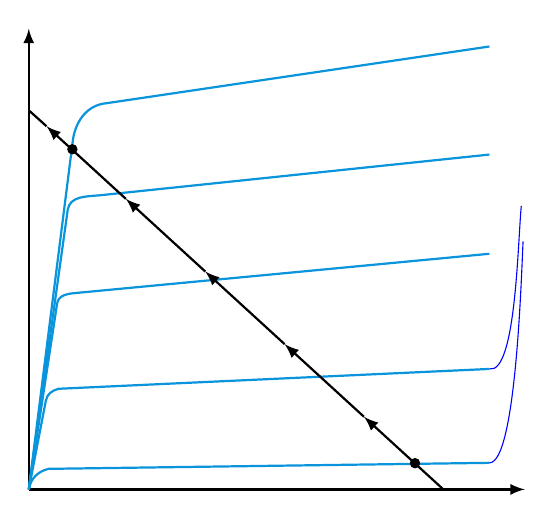
\begin{tikzpicture}[scale=0.45]
    %\node[anchor=south west,inner sep=0] (image) at (0,0) {\includegraphics[width=0.9\textwidth]{ImmaginiBJT/provacarattbjt.PNG}};
   % \begin{scope}[x={(image.south east)},y={(image.north west)}]
     %   \draw[help lines,xstep=.1,ystep=.1] (0,0) grid (1,1);
     %   \foreach \x in {0,1,...,9} { \node [anchor=north] at (\x/10,0) {\x}; }
     %   \foreach \y in {0,1,...,9} { \node [anchor=east] at (0,\y/10) {\y}; }
   % \end{scope}
    %disegno assi cartesiani
    \draw[thick, -latex](0,0)--(14,0);
    \draw[thick, -latex](0,0)--(0,13);
    %disegno grafici
    \draw[thick, thick,cyan!80!blue](0,0)to [in=195, out=80](0.55,0.58)--(13,0.75);
    \draw[thick, thick,cyan!80!blue](0,0)--(0.48,2.5) to [in=195, out=80](0.84,2.84)--(13,3.4);
    \draw[thick, thick,cyan!80!blue](0,0)--(0.8,5.25) to [in=185, out=80](1.4,5.55)--(13,6.65);
    \draw[thick, thick,cyan!80!blue](0,0)--(1.1,7.9) to [in=185, out=80](2,8.3)--(13,9.45);
    \draw[thick, thick,cyan!80!blue](0,0)--(1.25,9.9) to [in=185, out=80](2.2,10.9)--(13,12.5);

    \draw[blue](13,0.75)..controls (13.75,0.75) and (13.9,6).. (13.95,7);
    \draw[blue](13,3.4)..controls (13.75,3.25) and (13.8,7).. (13.9,8);
    %
    \pgfmathsetseed{2}
     \draw(11.6,0)--+(0.1,0) coordinate (i);
     \foreach \i in {1,2,3,4,5} { 
    \draw[black,thick,, -latex] (i)  
      -- ++(-2.24,2.05) coordinate(i); 
    }
    \draw[black,thick,](11.7-2.24*5, 2.05*5)--(0,10.7);

    \draw[fill] (10.9,0.74) circle (0.13 cm);
    \draw[fill] (1.23,9.6) circle (0.13 cm);
\end{tikzpicture}
\end{figure}
%
Come visto in precedenza:
\begin{align}
    I_B &= \dfrac{Q_B}{\tau_0} \nonumber\\
    I_C &= \dfrac{Q_B}{\tau_T} \nonumber
\end{align}
%
dove $Q_B$ e è la carica in eccesso accumulata nella base e $\tau_0$ la vita media dei portatori minoritari nella base.
Da ricordare che che la base è quasi-neutra, per cui le popolazioni in eccesso di elettroni e lacune sono uguali.
Conosco inoltre:
%
\begin{equation}
    \beta=\dfrac{I_C}{I_B}=\dfrac{\tau_0}{\tau_T} \nonumber
\end{equation}
%
In condizioni dinamiche l'equazione $I_B$ può
essere estesa in modo da tener conto delle variazioni della carica in eccesso. \\
Si ottiene l'equazione di controllo di carica
%
\begin{equation}
    I_B(t) = \dfrac{Q_B}{\tau_0} + \dfrac{dQ_B(t)}{dt}
\end{equation}
%
Si consideri un BJT (ad emettitore comune) inizialmente OFF. \\
Entrambe le giunzioni sono
polarizzate inversamente e quindi non vi è carica in eccesso nella base; la corrente
di base è praticamente nulla.\\
Supponiamo che al tempo $t = 0$ la corrente di base sia portata da zero ad un valore $I_{B1}$ sufficiente a saturare il dispositivo. \\
La corrente $I_{B1}$ inietta nella base una popolazione di lacune in eccesso, che rendono la
base carica positivamente e abbassano la barriera base-emettitore richiamando così
elettroni dall'emettitore. \\
Dopo un brevissimo transitorio iniziale (che si esaurisce
in un tempo $t_{in}$ dell'ordine del tempo di transito) nel quale le cariche iniettate
diffondono nella base e danno luogo alla distribuzione lineare di carica tipica della
zona attiva, il transistore esce dalla zona di interdizione ed entra in zona attiva
diretta . Una volta in zona attiva diretta, la carica iniettata in
eccesso dal lato emettitore continua ad aumentare per compensare la carica in
eccesso iniettata dalla corrente di base; fino a che tale compensazione non ha
avuto luogo la barriera base-emettitore non può alzarsi nuovamente limitando il
flusso di cariche iniettate.
Il tempo t; necessario a stabilire nella base una carica in eccesso Q e alimentando il transistore con una corrente di base Ip, si valutà integrando la $I_B$;
Maneggiando $I_B$ trovo che

\begin{equation}
    \int_0^{Q_B} \dfrac{\tau_0 }{\tau_0 I_{B1}-Q_B'} dQ_B'= \int_0^t dt
\end{equation}
%
da cui:
%
\begin{equation}
    t=\tau_0 \cdot \log{\left[ \dfrac{\tau_0 I_{B1}}{\tau_0 I_{B1}-Q_B}\right]}
\end{equation}
%
Ora sono in grado di calcolare la carica $Q_B$ accumulata nel tempo $t$:
\begin{equation}
    Q_B= I_{B1} \cdot \tau_0 \cdot \left[ 1- e^{-\frac{t}{\tau_0}}\right]
\end{equation}
%
\begin{figure}[h]
    \centering
    \begin{tikzpicture}
        
    \end{tikzpicture}
    \caption{Caption}
    \label{fig:enter-label}
\end{figure}
%
Poiché la situazione che stò analizzando è dinamica, non è vero che la corrente di collettore
è proporzionale alla corrente di base attraverso il parametro $\beta$. \\
Peraltro prendendo la formula di $I_C$ riportata all'inizio, possiamo vedere come la carica iniettata nella base cresce, la corrente di collettore creace a sua volta nel tempo spostando il punto di lavoro dinamico del transistore lungo la retta di carico di uscita. Per corrente di collettore sufficientemente elevata la tensione
collettore-emettitore sì abbassa al punto da fare entrare il transistore nella zona
di saturazione. Chiamiamo $I_{cs}$ tale corrente di collettore e definiamo $t_S$ come il
tempo necessario a raggiungere l'innesco della saturazione, ossia $I_c = I_{cs}$. Si ha, tenendo presente che $Q_B=\tau_t I_C=\dfrac{\tau_0 I_C}{\beta}$:
\begin{equation}
    t_s = \tau_0 \log{\left[ \dfrac{\beta I_{B1}}{\beta I_{B1}-I_{CS}}\right] \tikzmark{a}} 
\end{equation}

L'equazione precedente fornisce il tempo necessario alla commutazione di
un transistore alimentato da una corrente di base $I_{B1}$, con tempo di vita medio
dei portatori in base $\tau_0$, e caricato in modo tale da richiedere, per la saturazione, una corrente di collettore $I_{CS}$. Detta $I_{BS} = I_{CS}/\beta$ la corrente di base DC
corrispondente alla polarizzazione di collettore $I_{CS}$, sì ha che: 

\begin{enumerate}
    \item Per $I_{B1}<I_{BS}$ non ha soluzioni reali, ossia la corrente di collettore
non raggiunge mai $I_{DS}$. Questo non è sorprendente, perché non è possibile
che il transistore, alimentato in condizioni stazionarie da $I_{B1} < I_{BS}$, presenti
una corrente di collettore $\beta I_{B1}=I_{CS}=\beta I_{BS}$.
\item Per $I_{B1} = I_{BS}$ il tempo di commutazione è infinito, ossia la corrente di base
è appena sufficiente a fornire la corrente di collettore voluta. 

\item Per $I_{B1} > I_{BS}$, ossia quando la corrente di pilotaggio è maggiore della corrente
statica necessaria a sostenere $I_{CS}$, il tempo di commutazione è finito e tanto
più breve quanto più è elevata $I_{B1}$. 
\end{enumerate}
Per ridurre il tempo di commutazione ci sono diverse strade:
\begin{enumerate}
    \item Rendere minimo il tempo di vita medio $\tau_0$. Questo effetto pùò essere ottenuto
drogando la base con sostanze opportune che fungono da centri di ricombinazione, ad esempio con Au. 
\item Aumentare l'amplificazione di corrente. Questa seconda condizione si oppone
peraltro alla prima, poiché $\beta$ è direttamente proporzionale alla vita media. Sì
osservi che i criteri di progetto di ùun transistore per commutazione coincidono, per quanto riguarda il $\beta$ elevato, con quelli di un transistore usato come
amplificatore. 

\item aumentare la corrente di pilotaggio:
\begin{equation}
    I_C=\dfrac{Q_B}{\tau_t}=\dfrac{I_{B1}\tau_0}{\tau_t}\left[ \-e^{-t/\tau_0}\right]
\end{equation}
per cui, a parità di altre condizioni, il valore di $I_{CS}$ è raggiunto tanto più
rapidamente quanto è più elevato $I_{B1}$. 
\end{enumerate}
............
Dal punto di vista esterno l'innesco della saturazione stabilizza il punto di lavoro
del transistore per alti valori di corrente di collettore e bassi valori della tensione collettore-emettitore. Tenendo presente che in saturazione $V_{CE} \approx 0$, per un
transistore alimentato da una batteria di valore $V_{CC}$ e con resistenza serie di emettitore $R_3$ 
\begin{figure}
    \centering
    \begin{circuitikz}
        \draw (0,0) node[npn,anchor=B](npn){};
        \draw(npn.E) --++(0,-1) to node[tlground]{}++(0,0);
        \draw(npn.C) to [R,l_=$R_3$]++(0,1.5)--++(-0.75,0) coordinate(V);
        \draw(V) to [short,-*]++(0,+0.5)node[right]{$V_{CC}$};
        \draw(V)--++(-0.75,0) to [R,l_=$R_2$]++(0,-1.5)--++(0,-0.55)coordinate(b);
        \draw(b)-|(npn.B);
        \draw(b) to [R,l_=$R_1$]++(0,-1.55) to node[tlground]{}++(0,0);
    \end{circuitikz}
    \caption{Caption}
    \label{fig:enter-label}
\end{figure}
si ha $I_{CS} \approx V_CC/R_3$. Sì vede quindi che la corrente di collettore in grado di saturare il
transistore dipende essenzialmente da come il transistòre è caricato.
Il transitorio di commutazione non si esaurisce però all'innesco della saturazione, ossia quando la corrente di collettore si stabilizza in un intorno di $I_{CS}$. Vi
è un secondo transitorio, detto transitorio di sovrasaturazione, che influenza la distribuzione interna di carica del dispositivo. Infatti, quando il transistore esce
dalla zona attiva, la tensione base-collettore diviene positiva e anche la relativa
giunzione, polarizzata direttamente, comincia a iniettare portatori nella base. Il
grado di polarizzazione diretta raggiunto dalla giunzione collettore-base dipende
dalla struttura della rete che carica il transistore all'uscita e all'ingresso, e il profilo
finale della carica in eccesso nella base è mostrato nella Figura 13.27. \\
\begin{figure}[hbt!]
    \centering
    \includegraphics[width=0.5\textwidth]{Immagini/imm30.10.2023/transitorio ON-OFF.png}
    \caption{transitorio OFF-ON distribuzione di carica in eccesso nella base}
    \label{fig:transitorio OFF-ON distribuzione di carica in eccesso nella base}
\end{figure}
\\
Pertanto in saturazione vi è iniezione di portatori dall'emettitore nella base
e dalla base nell'emettitore (trascurabile se il drogaggio dell'emettitore è molto
maggiore di quello della base) come in zona attiva diretta, ma anche iniezione
di portatori dal collettore alla base e dalla base al collettore, dominante perché
la base è di solito più drogata del collettore. La corrente di base può pertanto
scriversi, dall'innesco della saturazione in poi: 

\begin{equation}
    I_B(t) = \dfrac{Q_{BS} + Q_{BSS}}{\tau_0} + \dfrac{dQ_{BSS}}{dt}
\end{equation}
dove $Q_{BS}$ è la carica all'innesco della saturazione, $Q_{BSS}$ la carica di sovrasaturazione iniettata dal collettore nella base. Si suppone che
nell'ultima fase del transitorio (la sovrasaturazione) la $Q_{BS}$ non cambi ulteriormente, perché poco influenzata dalla tensione base-collettore, mentre aumenti la
$Q_{BSS}$. Sì è anche supposto che la vita media delle cariche iniettate dal lato collettore sia circa uguale a quella delle cariche iniettate dal lato emettitore, anche se
questo non è a rigore vero.L'andamento nel tempo della carica di sovrasaturazione può ricavarsi in modo analogo a quanto visto per la carica di
saturazione; si ottiene: 

\begin{equation}
    Q_{BSS}(t)= \tau_0 \left[ I_{B1}- \dfrac{Q_{BS}}{\tau_0}\right] \cdot \left[ 1-  e^{-\dfrac{t-t_s}{\tau_0}}\right ]   t>t_s
\end{equation}
Anche se il comportamento del transistore non cambia esternamente dalla saturazione alla sovrasaturazione, la carica accumulata $Q_{BSS}$ deve essere eliminata in fase di commutazione ON-OFF; pertanto, la commutazione di apertura è inifluenzata dal valore di $Q_{BSS}$
%
\subsection{commutazione ON-OFF}
Considero sempre un transistor npn. I ragionamenti per studiare la commutazione ON->OFF di un transistor è uguale a quella fatta per la commutazione OFF->ON ma si percorrono i passi a ritroso.
\begin{figure}
    \centering
    \includegraphics[width=0.5\textwidth]{Immagini/imm30.10.2023/transitorio ON-OFF.png}
    \caption{transitorio ON-OFF distribuzione di carica in eccesso nella base}
    \label{fig:transitorio ON-OFF distribuzione di carica in eccesso nella base}
\end{figure}
%
\begin{center}
    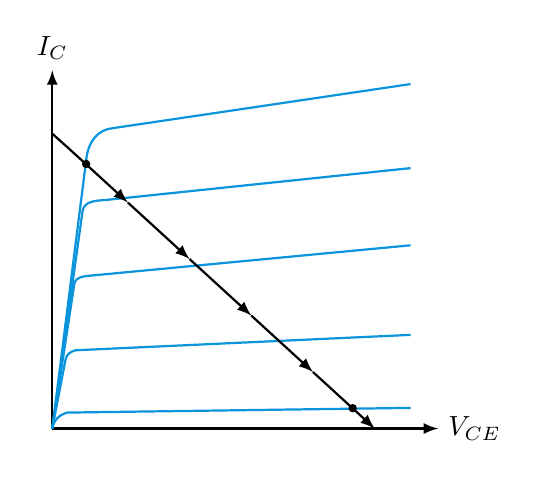
\begin{tikzpicture}[scale=0.35]
    %disegno assi cartesiani
    \draw[thick, -latex](0,0)--(14,0) node[right] {$V_{CE}$};
    \draw[thick, -latex](0,0)--(0,13) node[above] {$I_C$};
    
    %disegno grafici
    \draw[thick, thick,cyan!80!blue](0,0)to [in=195, out=80](0.55,0.58)--(13,0.75);
    \draw[thick, thick,cyan!80!blue](0,0)--(0.48,2.5) to [in=195, out=80](0.84,2.84)--(13,3.4);
    \draw[thick, thick,cyan!80!blue](0,0)--(0.8,5.25) to [in=185, out=80](1.4,5.55)--(13,6.65);
    \draw[thick, thick,cyan!80!blue](0,0)--(1.1,7.9) to [in=185, out=80](2,8.3)--(13,9.45);
    \draw[thick, thick,cyan!80!blue](0,0)--(1.25,9.9) to [in=185, out=80](2.2,10.9)--(13,12.5);
    
    % Linee di transizione
    \pgfmathsetseed{2}
    \draw(11.6,0)--+(0.1,0) coordinate (i);
    \foreach \i in {1,2,3,4,5} { 
        \draw[black,thick, latex-] (i) -- ++(-2.24,2.05) coordinate(i); 
    }
    \draw[black,thick](11.7-2.24*5, 2.05*5)--(0,10.7);
    
    % Punti di interesse
    \draw[fill] (10.9,0.74) circle (0.13 cm);
    \draw[fill] (1.23,9.6) circle (0.13 cm);
\end{tikzpicture}
\end{center}
%
In una prima fase, la diminuzione della corrente di base diminuisce la carica positiva in eccesso nella base, ossia carica la base negativamente. \\
Il primo effetto è l'aumento della barriera base-collettore, che porta alla riduzione della carica iniettata dal collettore, e quindi alla scomparsa
della carica di sovrasaturazione con costante di tempo dell'ordine di $\tau_0$. Venendo
a mancare la carica iniettata dal collettore nella base, la carica di sovrasaturazione
si esaurisce esponenzialmente secondo la legge: 

Deve sparire $Q_{BSS}(t)$:
%
\begin{equation}
    Q_{BSS}(t)=Q_{BSS}(0) \cdot e^{-\frac{t}{\tau_0}}
\end{equation}
%
Con $Q_{BSS}(0)$ è la carica al tempo zero.\\
Il tempo per spegnerlo dipende da t0 e $\tau_0$, ovvero da quanto lo abbiamo caricato.\\
In totale si apsetta il tempo tss.\\
%
Definiamo come tss il tempo necessario a eliminare (o a ridurre considerevolmente) la carica di sovrasaturazione. Quando questo avviene, il transistore entra nella
zona attiva. Peraltro, poiché la corrente di base non è in grado di sostenere l'elevata corrente di collettore corrispondente all'innesco della saturazione, la carica in
eccesso iniettata dalla giunzione emettitore-base comincia a diminuire. Il valore iniziale è pari a Qps, mentre il valore finale è dato dalla relazione ITp2 = QB (00)/7oRisolvendo l'equazione a controllo di carica (13.24) con Ig = Ip2, tempo iniziale pari a tss e le condizioni iniziali e finali citate in precedenza, si ottiene: 
%

%
\begin{equation}
    Q_B(t)=\tau_0 \cdot I_{B2} \left[ 1-e^{-\dfrac{t-t_{ss}}{\tau_0}}\right] + Q_{BS} \cdot e^{-\dfrac{t-t_{ss}}{\tau_0}} \text{, } t \gg t_ss
\end{equation}
%
tale equazione dipende da $I_{B2}$ e se ne possono identificare 2 valori.\\

Quando la carica Q si annulla, il transistore entra nella regione di interdizione.
A seconda del valore di Ig2 si hanno tre distinte condizioni: 


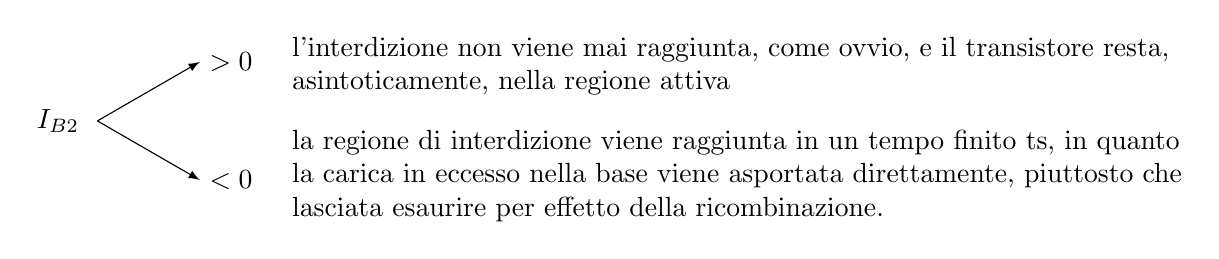
\begin{tikzpicture}
\node at (-0.5,0) []{$I_{B2}$};
\draw[-latex] (0,0) -- ++ (1.3,+0.75) node[align= left,right] {$>0$};
\node at (2.35,+0.7) [align=left,right]{l'interdizione non viene mai raggiunta, come ovvio, e il transistore resta,\\ asintoticamente, nella regione attiva};

\draw[-latex] (0,0) -- ++ (1.3,-0.75) node[right] {$< 0$ };
\node at (2.35,-0.7) [align=left,right]{la regione di interdizione viene raggiunta in un tempo finito ts, in
quanto \\la carica in eccesso nella base viene asportata direttamente, piuttosto
che \\lasciata esaurire per effetto della ricombinazione. };
\end{tikzpicture}

%
In conclusione quindi la corrente di base e di collettore in un transitorio di apertura
e chiusura hanno l'aspetto mostrato nella Figura 13.29. Da un punto di vista
pratico, si definiscono come tempi caratteristici il tempo di salita t- e il tempo di
discesa t;. Questi sono definiti come segue, detta Alc la variazione di corrente
fra l'interdizione e la saturazione: 
Vogliamo vedere il transitorio a fronte di una commutazione
\begin{itemize}
    \item $t_r$ è il tempo necessario a passare dal $10\%$ di $\Delta I_C$ al $90\%$ di $\Delta I_C$;
    \item $t_f$ è il tempo necessario a passare dal 90\% di $\Delta I_C$ al 10\% di $\Delta I_C$. 
\end{itemize}
%
Generalmente il tempo di salita è grande rispetto al tempo di ritardo iniziale tin
necessario per passare dall'interdizione all'innesco della regione attiva. Una stima
del tempo di salita valida quando la commutazione viene pilotata da una corrente
di base appena sufficiente (Ig2 \& Ics/B per il transitorio OFF-ON e Ig2 \& 0 per
il transitorio ON-OFF) è: 
%
\begin{equation}
    t_r \approx 2.2 \tau_0
\end{equation}
pg609 spiega come trova il valore 2.2
%
In conclusione quindi il tempo di commutazione di un transistore bipolare
è proporzionale alla vita media dei portatori nella base. Per tale motivo, nei
transistori per commutazione si usa talvolta drogare con oro la base allo scopo di
abbassare 70 e di rendere così più rapida la commutazione del dispositivo. 

\begin{tikzpicture}
    %grafico commutazione
    %disegno asse x
    \draw[-latex](0,0)--(6,0)node[right]{t};
    %disegno asse y
    \draw[-latex](0,0)--(0,2.5)node[left]{$I_B$};
    %grafico commutazione
    \draw[thick](0,0)--++(1.5,0)--++(0,1)--++(3,0)--++(0,-1)--++(1.5,0);
    
    %grafico transizione
    %disegno asse x
    \draw[-latex](0,-3)--(6,-3)node[right]{t};
    %disegno asse y
    \draw[-latex](0,-3)--(0,-0.5)node[left]{$I_B$};
    %grafico commutazione
    \draw[thick](0,0)--++(1.5,0)--++(0,1)--++(3,0)--++(0,-1)--++(1.5,0);
\end{tikzpicture}
I tempi sono tali per cui $tr=tf \approx 2.2\tau_0$\\
44\\
Si può dire che è necessario trovare un compromesso tra Vce->0 e velocità  di commutazione. Maggiori saranno le Ib, maggiori saranno le cariche iniettate in base e quindi maggioresarà il tempo di smaltimento di queste ultime.\\
Nel caso di un bjt asimmetrico, come collettore poco drogato, la carica di $Q_{BSS}$ è poca (bjt più veloce) ma Vce diverso da 0 perciò non esistono condizioni di cortocircuitoequivalente tra C ed E\\
\\
Vedendo la sezioni del BJT, si ha:
%
\begin{figure}[hbt!]
    \centering
    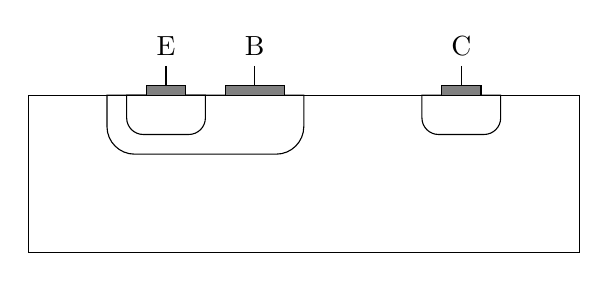
\begin{tikzpicture}
        \draw(0,0) rectangle++(7,2);
        %base
        \draw(1,2) --
          ++(2.5,0) {[rounded corners=10]--++(0,-0.75)--++(-2.5,0)} 
          -- cycle {};
        %emettitore
        \draw(1.25,2) --
          ++(1,0) {[rounded corners=6] --
          ++(0,-0.5) --
          ++(-1,0)} 
          -- cycle
          {};
        %collettore
        \draw(5,2) --
          ++(1,0) {[rounded corners=6] --
          ++(0,-0.5) --
          ++(-1,0)} 
          -- cycle
          {};
        %metallizzazioni
        \draw[fill=gray](1.5,2) rectangle++(0.5,0.125)
        (1.75,2.125)--++(0,0.25) node[anchor=south]{E};
        \draw[fill=gray](2.5,2) rectangle++(0.75,0.125)
        (2.875,2.125)--++(0,0.25) node[anchor=south]{B};
        \draw[fill=gray](5.25,2) rectangle++(0.5,0.125)
        (5.5,2.125)--++(0,0.25) node[anchor=south]{C};

    \end{tikzpicture}
    \caption{Sezione BJT}
    \label{fig:sezione BJT}
\end{figure}
%
Spesso c'è un'ulteriore zona p ed un buffer n+.\\
La zona p sono fatte per isolamento n+ è lo strato sepolto per creare n+ e p- una giunzione OFF che impedisce alle correnti di andare sott e le correnti faranno il giro.

\begin{figure}[hbt!]
    \centering
    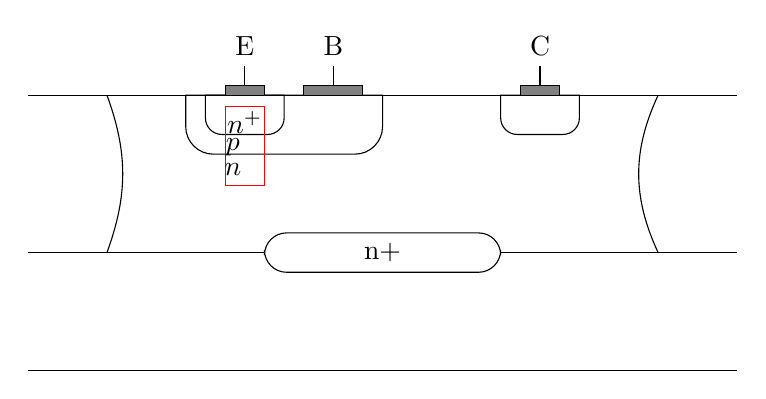
\begin{tikzpicture}
        \draw (0,0) to[in=290, out=70] (0,2);
        \draw (-1,2) -- (8,2);
        \draw (7,2) to[in=115, out=245] (7,0);
        \draw (-1,0) -- (2,0);
        \draw [rounded corners = 8pt]  (2,-0.25) rectangle ++(3,0.5) node[pos=.5]{n+};
        \draw (5,0) -- (8,0);
        \draw (-1,-1.5) -- (8,-1.5);
        
        %rectangle++(7,2);
        %base
        \draw(1,2) --
          ++(2.5,0) {[rounded corners=10]--++(0,-0.75)--++(-2.5,0)} 
          -- cycle {};
        %emettitore
        \draw(1.25,2) --
          ++(1,0) {[rounded corners=6] --
          ++(0,-0.5) --
          ++(-1,0)} 
          -- cycle
          {};
        %collettore
        \draw(5,2) --
          ++(1,0) {[rounded corners=6] --
          ++(0,-0.5) --
          ++(-1,0)} 
          -- cycle
          {};
        %metallizzazioni
        \draw[fill=gray](1.5,2) rectangle++(0.5,0.125)
        (1.75,2.125)--++(0,0.25) node[anchor=south]{E};
        \draw[fill=gray](2.5,2) rectangle++(0.75,0.125)
        (2.875,2.125)--++(0,0.25) node[anchor=south]{B};
        \draw[fill=gray](5.25,2) rectangle++(0.5,0.125)
        (5.5,2.125)--++(0,0.25) node[anchor=south]{C};

        %BJT
        \draw[red] (1.5,1.85) rectangle++(0.5,-1) ;
        \node at (1.75,1.65) []{$n^+$};
        \node at (1.6,1.34) []{$p$};
        \node at (1.6,1.05) []{$n$};
    \end{tikzpicture}
    \caption{Sezione BJT}
    \label{fig:sezione BJT}
\end{figure}
Quello che importa è la dimensione dell'area del transistor perchè il transistor si basa sulla corrente uscente dall'emettitore. perciò tale dimensione è quella che governa la corrente.\\. visto dall'alto si ha: 
%
\begin{figure}[hbt!]
    \centering
    \begin{tikzpicture}
        \draw(0,0) rectangle++(8,3);

        \draw (1.5,0.75) rectangle++(1,1.5) node[pos=0.5]{E};
        \draw (1,0.5) rectangle++(4,2) node[pos=0.5]{B};
        \draw (6,0.75) rectangle++(1,1.5) node[pos=0.5]{C};

        \draw[pattern=north east lines, pattern color= red](1.5,0.75) rectangle++ (1,1.5) node[anchor= south east, red]{$A_e$};
    \end{tikzpicture}
    \caption{Caption}
    \label{fig:enter-label}
\end{figure}
%
\subsubsection{Alte iniezioni}
Per analizzare meglio il comportamento del BJT in caso di alte iniziezioni, comincio scrivendo l'equazione della corrente di elettroni che entra in base :
\begin{align}
    J_n &=-q\cdot n_p \cdot \mu_n \cdot \dfrac{d\phi_n}{dx}
\end{align}
Dove $n_p$ è la concentrazione di elettroni di base (che è un semiconduttore p), $\Phi_n$ è il potenziale associato al quasi livelli di fermi del lato n. Si considera quindi la presenza di una corrente di deriva dovuta al campo elettrico descritto come derivata del livello di quasi fermi dell'emettitore.
In base, il quasi livello di fermi delle lacune è pressochè costante perciò posso dire che $\dfrac{d\phi_p}{dx} \approx 0$.\\
Ora applico uno stratagemma matematico. Sommo $Jn$
Applico uno stratagemma matematico. sommo i due potenziali sapendo che tando quello della basse è praticamente zero:
%
\begin{align}
    J_n &=-q\cdot n_p \cdot \mu_n \cdot \dfrac{d[-(\phi_p-\phi_n)]}{dx}\\
\end{align}
%
dove ricordo che in un diodo vale la relazione:
%
\begin{equation}
    \phi_p -\phi_n = \dfrac{k_B T}{q}\ln{\left[  \dfrac{n_p P_p}{{n_i}^2}\right]}
\end{equation}
\begin{exbox}
    \begin{itemize}
        \item $n_p$ è il numero di elettroni, portatori minoritari in base
        \item $P_p$ è il numero di lacune, portatori maggioritari, in base
    \end{itemize}
\end{exbox}
%
unendo tutto questo con la relazione di Einstein $D_n = \mu_n \cdot V_T$, ottengo: 
%
\begin{equation}
    J = q D_n \dfrac{n_i^2}{P_p} \dfrac{d}{dx}\left[ \dfrac{n_p \cdot P_p}{n_i^2}\right]
\end{equation}
%
Se considero l'ipotesi di un semiconduttore molto drogato è questo comporta un'importante considerazione sui livelli energetici:\\
Il legame tra un semiconduttore drogato e i livelli nella banda proibita è che le impurità introdotte durante il drogaggio creano questi livelli energetici all'interno della banda proibita. Questi livelli possono agire come stati di transizione per gli elettroni, consentendo loro di saltare tra la banda di valenza e la banda di conduzione più facilmente rispetto a un semiconduttore intrinseco
veceversa.\\
Siccome i livelli in banda aumenta, questo si può vedere come un restringimento del GAP ad un valore $E_g' <E_g$. Ma questo comporta nell'avere un $n_{ie}>n_i$. allora la formula diventerà:
\begin{equation}
    J = q D_n \dfrac{n_{ie}^2}{P_p} \dfrac{d}{dx}\left[ \dfrac{n_p \cdot P_p}{n_i^2}\right]
\end{equation}
\begin{exbox}
    per le lacune iniettate verso lemettitore. si avrà:
%
\begin{equation}
    J = - q D_p \dfrac{n_i^2}{n_n} \dfrac{d}{dx}\left[ \dfrac{n_n \cdot P_n}{n_i^2}\right]??
\end{equation}
\end{exbox}
%
Riscrivo l'equazione in modo diverso:
\begin{equation}
    J_n \cdot \dfrac{P_p}{ q D_nn_{ie}^2} =\dfrac{d}{dx}\left[ \dfrac{n_p \cdot P_p}{n_i^2}\right]
\end{equation}
Se ora lo integro per tutta l'estensione della base, trovo:
%
\begin{equation}
    J_n \int_0^{W_B} \dfrac{P_p}{D_n \cdot n_{ie}^2}dx = \left.\dfrac{n_p \cdot P_p}{n_{ie}^2}\right|_{W_B} -\left. \dfrac{n_p \cdot P_p}{n_{ie}^2}\right|_{x=0}
\end{equation}
Dove $\left.\dfrac{n_p \cdot P_p}{n_i^2}\right|_{W_B}= -\dfrac{n_p(W_B)P_p(W_B)}{n_{ie}^2(W_B)} \approx 0 $ perchè la concentrzione di elettroni nel punto Wb è praticamente nulla visto che appena un elettrone arriva in tale zona, esso viene subito spinto verso il collettore. si ha quindi:
\begin{equation}
   J_n \int_0^{W_B} \dfrac{P_p}{D_n \cdot n_{ie}^2}dx =-\left. \dfrac{n_p \cdot P_p}{n_{ie}^2}\right|_{x=0}= -\dfrac{n_p(0)e^{\frac{V_{BE}}{V_T}}\ P_p(0)}{n_{ie}^2} 
\end{equation}
dove $n_p(0)$ è la quantità di elettroni in p a riposo cioè in assenza di tensione applicata (vbe=0).\\

--??\\

Nei transistor moderni, la base dei BJT è drogato in modo tale da avere un picco nella giunzione base eemttitore.Se tale picco risulta largo, cioè la concentrazione (in questo punto) di portatori maggiroitari (lacune) è molto più grande di quelli minoritari iniettati, NON vi è ricombinazione sufficente quindi $P_p(0)\approx P_{p0}(0)=N_{AB}$
\begin{ricevimento}
    ?????? cosa c'è scritto sopra?
\end{ricevimento}

\begin{equation}
    J_n \int_0^{W_B} \dfrac{P_p}{D_n \cdot n_i^2}dx = -\dfrac{n_{p0}(0)P_{p0}(0)}{n_{ie}^2(0)} e^{\frac{V_{BE}}{V_T}}= -\dfrac{n_{ie}^2(0)}{n_{ie}^2(0)} e^{\frac{V_{BE}}{V_T}}
\end{equation}
dove ho scritto nie(x) a causa del forte drogaggio.\\
Si è assunto che $np0(0)=Pp0(0)=n_{ie}^2$ perchè di fatto è così per quanto visto dalla legge di azione di massa.
allora:
\begin{equation}
    J_n = - \dfrac{q \exp\left[ V_{BE}/V_T\right]}{\int_0^{W_B} \dfrac{P_P}{D_n n_{ie}^2}dx}
\end{equation}
Questa rappresenta la corrente di elettroni in base.\\
Se Pp è costante e pari ad $N_{AB}$ come nel modello di ebers moll si ottiene la stessa espressione che si trovava in precedenza. QUesto modello tiene conto delel alte iniezioni con Pp, infatti se $Pp>N_AB$, allora la corrente subisce una riduzione. guardando le formule:\\
allora la corrente di collettore sarà:
\begin{equation}
    I_C=A_E |J_{n}| =A_E |J_C|= \dfrac{qA_E e^{B_{be}/V_T}}{\int_0^{W_b}ni^2(\dfrac{P_p}{D_n \ n_{ieb}^2})dx}n_i^2
\end{equation}
Con AE l'area di emettitore. Se considero $I_{C0}=\dfrac{qn_i^2}{\int_0^{W_b}n_i^2(\dfrac{P_p}{D_n\ n_{ieb}^2})dx}=\dfrac{qn_{ieb}^2}{GB}$ dove GB è detto numero di gummel.
\begin{equation}
    G_B=\int_0^{Wb}ni^2\dfrac{P_p}{D_n\ n_{ie}^2}/dx
\end{equation}
allora:
\begin{equation}
    I_C=A_E J_{C0}e^{V_{be}/V_T}
\end{equation}
\begin{equation}
    I_C=A_E |J_{nEB}| = -A_E \dfrac{qn_i^2}{G_B}e^{V_{be}/V_T}
\end{equation}

Da cancellare??\\
---------------------------\\

Nel caso di alte iniezioni varia la quantità di cariche maggioritarie in P talmente tanto che $P_p \neq N_A$.
La condizione $P_p =N_A$ vale sono per piccole iniezioni e $G_B=\dfrac{N_A W_B}{D{np}n_{iEB}^2}$.
Se gli elettroni in base diventato tantissimi allora le lacune vengono richiamate in base. si avrà un aumento di GB ed una diminuzione di IC

--grafici e formule...
%
Se Pp=cost=$N_A$ si ha $I_{c0}$ ricavata nelle eq precedenti.\\
GB cambia con le iniezioni.
\\
Per basse iniezioni $P_p=N_A$\\
\begin{equation}
    G_B=N_A \cdot W_{B}
\end{equation}
Negli altri casi cambia.\\
grafico\\
\begin{equation}
    J_C=q \, N_C \cdot v_{sat}
\end{equation}
%
Cosa succede poi? al lato del collettore

questo è detto effetto kirk\\
------------------------------------\\
\cleardoublepage
\subsubsection{Spostamento del collettore: effetto KIRK}
è un meccanismo che si smma a quello precedente.
La massima corrente che può sopportare il collettore è:
\begin{equation}
    J_C^{max}=qN_Cv_{sat}
\end{equation}
Questo è il limite della saturazione massima sopportabile.
\begin{figure}[hbt!]
    \centering
    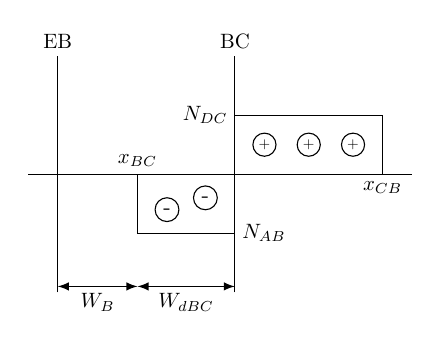
\begin{tikzpicture}[scale=0.75, transform shape]
    %disegno asse x
    \draw(-0.5,0)--(6,0);
    %sezione EB
    \draw(0,-2)--(0,2) node[anchor=south]{EB};
    %sezione BC
    \draw(3,-2)--(3,2)node[anchor=south]{BC};
    %disegno grafico
    \draw(1.35,0)rectangle(3,-1);
    \draw(3,0)rectangle(5.5,1);
    
    %disegno ioni fissi negativi
    \node[draw, circle, minimum size=1.8mm,scale=0.6] at (2.5,-0.4) {\scalebox{1.8}{-}};
    \node[draw, circle, minimum size=1.8mm,scale=0.6] at (1.85,-0.6) {\scalebox{1.8}{-}};
    %disegno ioni fissi positivi
    \node[draw, circle, minimum size=1.8mm,scale=0.4] at (3.5,0.5) {\scalebox{1.8}{+}};
    \node[draw, circle, minimum size=1.8mm,scale=0.4] at (4.25,0.5) {\scalebox{1.8}{+}};
    \node[draw, circle, minimum size=1.8mm,scale=0.4] at (5,0.5) {\scalebox{1.8}{+}};
    
    %label x e y
    \node at (1.35,0)[anchor=south]{$x_{BC}$};
    \node at (5.5,0)[anchor=north]{$x_{CB}$};
    \node at (3,1)[left]{$N_{DC}$};
    \node at (3,-1)[right]{$N_{AB}$};
    %freccie e label
    \draw[latex-latex] (0,-1.9) -- (1.35,-1.9) node[midway, below] {$W_B$};
    \draw[latex-latex] (1.35,-1.9) -- (3,-1.9) node[midway, below] {$W_{dBC}$};
    
    \end{tikzpicture}
    \caption{Caption}
    \label{fig:enter-label}
\end{figure}
%
Nel caso $V_{BE}>V_{th}$,se molti elettroni vengono iniettati in base dall'emettitore succederà, in primo luogo che questi portatori tenederanno a ridurre la regione degli ioni fissi. Questo primo effetto è l'equivalente di un aumento del drogaggio in base (WB aumenta).
Viceversa nel collettore, prima di essere raccolti gli elettroni caduti del pozzo di potenziale, danno come effetto equivalente quello di riduzione dei portatori di carica maggioritari e quindi dell'allargamento della regione di ioni fissi positivi.
questi due sono detti effetto KIRK.
%
\begin{figure}[hbt!]
    \centering
    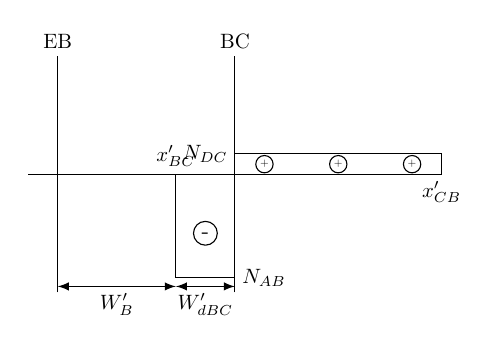
\begin{tikzpicture}[scale=0.75, transform shape]
    %disegno asse x
    \draw(-0.5,0)--(6,0);
    %sezione EB
    \draw(0,-2)--(0,2) node[anchor=south]{EB};
    %sezione BC
    \draw(3,-2)--(3,2)node[anchor=south]{BC};
    %disegno grafico
    \draw(2,0)rectangle(3,-1.75);
    \draw(3,0)rectangle(6.5,0.35);
    
    %disegno ioni fissi negativi
    \node[draw, circle, minimum size=1.8mm,scale=0.6] at (2.5,-1) {\scalebox{1.8}{-}};
    %disegno ioni fissi positivi
    \node[draw, circle, minimum size=1.8mm,scale=0.3] at (3.5,0.17) {\scalebox{1.8}{+}};
    \node[draw, circle, minimum size=1.8mm,scale=0.3] at (4.75,0.17) {\scalebox{1.8}{+}};
    \node[draw, circle, minimum size=1.8mm,scale=0.3] at (6,0.17) {\scalebox{1.8}{+}};
    
    %label x e y
    \node at (2,0)[anchor=south]{$x'_{BC}$};
    \node at (6.5,0)[anchor=north]{$x'_{CB}$};
    \node at (3,0.35)[left]{$N_{DC}$};
    \node at (3,-1.75)[right]{$N_{AB}$};
    %freccie e label
    \draw[latex-latex] (0,-1.9) -- (2,-1.9) node[midway, below] {$W'_B$};
    \draw[latex-latex] (2,-1.9) -- (3,-1.9) node[midway, below] {$W'_{dBC}$};
    
    \end{tikzpicture}
    \caption{Caption}
    \label{fig:enter-label}
\end{figure}
%
Se WB aumenta allora $\beta$ diminuisce. Inoltre l'apparente diminuzione del drogaggio del collettore contribuisce a diminuire anche la corrente di collettore massima (se $N_C \downarrow$ allota $J_C^{max} \downarrow$)
infatti la corrente di collettore operativa sarà minore di quello massimo ($J_C^{ops}<J_C^{max}$) tipicamente sarà il 30\% del valore massimo.\\
inoltre l'aumento di Wb comporta l'aumento di GB e quindi la diminuzione di IC
%
beta è il prodotto guadagno banda min 40..
\cleardoublepage
\subsection{Modello del BJT generico: il modello di Gummel-Poon}
Il seguente modello è usato dai vari CAD per simulare la risposta dei BJT al variare di $V_{BE}(t)$ e $V_{CE}(t)$.\\
Il modello circuitale è costruito sulla base del modello di Ebers-Moll con l'aggiunta di componenti che descrivono il comportamento reale quali, alte iniezioni, cariche nel transistor e resistene parassite
\begin{figure}[hbt!]
    \centering
    \includegraphics{Immagini/imm30.10.2023/30_10_BJT_GummelPoolModel.png}
    \caption{Modello di Gummel-Poon}
    \label{fig:Modello di Gummel-Poon}
\end{figure}
I due diodi rappresentano i termini che formano la $I_B$ a causa della tensione $V_{BE}$ e $V_{BC}$.\\
La capacità $Q_F$ è un componente dipendente dalla tensione messa per rappresentare l'andamento del trasporto di carica (io l'ho chiamato $Q_B$). questo condensatore e la sua tensione di controllo sono scelti in in modo tale che la sua carica immagazzinata sia uguale che serve a descrivere $Q_F=Q_B$ cioè la somma di tutte le lacune in eccesso immagazzinate nell'emettitore, nella base e nella regione di svuotamento tra i due.
\begin{exbox}
    introduco tempo di immagazzinamento (diverso dal tempo di transito):
    \begin{equation}
        \tau_F=\dfrac{Q_F}{I_C}
    \end{equation}
\end{exbox}
$Q_R$ è la componente duale di $Q_F$ che viene creato nella condizione di giunzione BC polarizzato direttamente.\\

Le capacità $C_{BE}$ e $C_{BC}$ sono le capacità di giunzione mentre la $C_{CS}$ è una capacità che si forma tra collettore e substrato 
%
\cleardoublepage
\subsection{Breakdown}
\begin{figure}[hbt!]
    \centering
    \includegraphics{Immagini/imm30.10.2023/BJT_RAD_breakdown.png}
    \caption{Caption}
    \label{fig:enter-label}
\end{figure}
Il breakdown nei BJT sono simili a quelli delle giunzioni p-n e in particolare si possono studiare due tipi di meccanismi di breakdown:
%
\begin{enumerate}
    \item Breakdown per perforazione diretta
    \item Breakdown per effetto valanga
\end{enumerate}
Sebbene la perforazione diretta sia uno dei meccanismi di breakdown, tale fenomeno diventa trascurabile se si considera che essa necessita di una tensione inversa generalmente molto più grande di quella necessaria a provocare l'effetto valanga. 
%
\begin{ripasso}[ripasso breakdown p-n]
Quando una giunzione di semiconduttore è polarizzata inversamente, si crea una barriera di potenziale attraverso la giunzione, che ostacola il movimento degli elettroni liberi nel semiconduttore N e delle lacune nel semiconduttore P attraverso la giunzione.

Se la tensione inversa applicata aumenta gradualmente, anche la larghezza della zona di svuotamento nella giunzione aumenta fino a quando, ad un certo punto, il campo elettrico che sussiste nella regione diventa talmente grande che gli elettroni nel semiconduttore N e le lacune nel semiconduttore P possono guadagnare abbastanza energia per superare la barriera di potenziale della zona di svuotamento, creando il brakdown.
\end{ripasso}
%
\cleardoublepage
\subsubsection{Breakdown BJT per perforazioen diretta}
Il breakdown del BJT per perforazione diretta avviene a seguito di una polarizzazione inversa $V_{BC}$ talmente alta da fare in modo che la regione di svuotamento B-C si allarghi fino a toccare la regione di svuotamento B-E.
In questa condizione la barriera di potenziale emettitore-base delle lacune viene influenzata anche dalla $V_{BC}$. Adesso servono piccoli incrementi di $V_{BC}$  per avere grandi incrementi di $I_C$
\begin{figure}[hbt!]
    \centering
    \includegraphics[width=0.5\textwidth]{Immagini/imm30.10.2023/30_10_BJT_breakdown punch.png}
    \caption{Caption}
    \label{fig:enter-label}
\end{figure}

\subsection{Breakdown BJT per effetto valanga}
L'unicità del breakdown del BJT per effetto valanga sta nel fatto che la tensione di breakdown che provoca il fenomeno dipende dalla configurazione del circuito:\\
%
\begin{itemize}
    \item \noindent\begin{minipage}{0.7\textwidth}
            modalità emettitore comune. Si applica una tensione $V_{CE}$ mentre la base è staccata e l'uscita è al collettore-emettitore del dispositivo).
            in questa configurazione la gionzione BC è polarizzata inversamente
            \end{minipage}
            \hfill%
            \begin{minipage}{0.2\textwidth}\raggedleft
                \begin{circuitikz}
                \draw(0,0) to [short,*-](0.25,0) node[npn,anchor=B](npn1){};
                \draw(npn1.C)--++(0,+0.35)--++(0.75,0) to [battery1,l=$V_{CE}$]++(0,-1.75)--++(-0.75,0) coordinate(m);
                \draw (npn1.E)--++(0,-0.55) node[tlground]{};
                
                % Add the current arrow and label
                  \draw[->, >=stealth, thick] (0,0.2) --++ (0.35,0) node[midway, above] {\small $ I_B=0$};
                  \draw[->, >=stealth, thick] (1.5,1) --++ (-0.55,0) node[midway, above] {\small $ I_C$};
                  \draw[->, >=stealth, thick] (0.75,-0.85) --++ (0,0.45) node[midway, left] {\small $ I_E$};
                \end{circuitikz}
            \end{minipage}

    \item \noindent\begin{minipage}{0.7\textwidth}
            modalità base comune (cioè con la base collegata , l'emettitore staccato  e l'uscita al collettore-base del dispositivo).\\
            la tensione $V_{BC}$ applicata in polarizzazione inversa. la corrente $I_{CB0}$ è la corrente della giunzione inversamente polarizzata.
            \end{minipage}
            \hfill%
            \begin{minipage}{0.2\textwidth}\raggedleft
                 \begin{circuitikz}                
                  \draw(0,0) to [short,*-](0.25,0) node[npn,anchor=E,yscale=-1,rotate=-90](npn2){};
                    \draw(npn2.C)--++(0.75,0) to [battery1,l=$V_{CB}$]++(0,-1.10)--++(-1.3,0) coordinate(m);
                    \draw (npn2.B)--++(0,-0.65) node[tlground]{};
                    
                    % Add the current arrow and label
                  \draw[->, >=stealth, thick] (0,0.2) --++ (0.35,0) node[midway, above] {\small $ I_E=0$};
                  \draw[->, >=stealth, thick] (1.95,0.2) --++ (-0.6,0) node[midway, above] {\small $ I_C$};
                  \draw[->, >=stealth, thick] (1,-0.9) --++ (0,0.4) node[midway, right] {\small $ I_B$};
                \end{circuitikz}
            \end{minipage}
\end{itemize}


%
Nei transistor BJT in configurazione RAD, il breakdown si verifica a seguito dell'effetto valanga che interviene nella giunzione base collettore che è polarizzata inversamente.
Il breakdown non si verifica tra emettitore e base perchè tale giunzione è polarizzata direttamente, quindi , è sede di una corrente di portatori.

%
\paragraph{Configurazione CB}\mbox{}\\
%
Quando il transistor è polarizzato in configurazione emettitore aperto, la corrente $I_{CB0}$ quando raggiunge il breakdown viene moltiplicato per un fattore di moltiplicazione M e diventa $M \cdot I_{CB0}$\\
 Dove $M(V)=\dfrac{1}{1-\left( V_{CB}/BV_{CB0}\right)^m}$
    è una formula empirica chiamata fattore di moltiplicazione a valanga (o guadagno per effetto moltiplicazione a valanga). Dentro la funzione empirica M posso identificare alcuni parametri:
    \begin{enumerate}
        \item $V_{CB}$ è la tensione in polarizzazione inversa;
        \item $BV_{CB0}$ è la tensione di breakdown in configurazione common base (emettitore aperto);
        \item $m$ è un parametro che dipende dal pateriale e dalla sua resistività. $m:3 \div 6$.
    \end{enumerate}
%
\paragraph{Configurazione CE}\mbox{}\\
%
Quando il transistor è polarizzato in configurazione base aperta si possono fare due considerazioni

\begin{enumerate}
    \item la corrente in uscita dalla regione di carica spaziale del collettore è M volte la corrente di quella che entra nella regione di carica spazionale nella base:
    %
    \begin{equation}
        J_n(W_B + W_{dCB}) = M J_n(W_B) \text{, } \, M>1
    \end{equation}
    %
    
    \item Ricordo il parametro del guadagno di corrente in CB $\alpha_0$ che è la variazione della $I_C$ sulla variazione di $I_E$.\\
    Io ho studiato il caso semplice in cui $\alpha=\gamma \cdot b$, ottenuta nella condizione di effetto valanga trascurabile (quando $M \approx 1$) ma in realtà, nel caso generale vale :
    %
    \begin{equation}
        \alpha_0=\dfrac{dI_C}{d(-I_E)}=\gamma \cdot b \cdot M
    \end{equation} 
\end{enumerate}
%
\begin{exbox}[come si è ricavato $\alpha_0$?]
Si parte considerando la corrente di collettore. Essa è uguale alla corrente di elettroni che escono dalla regione di svuotamento della giunzione B-C
\begin{equation*}
    I_C= A_C \,J_n(W_B+W_{dBC})
\end{equation*}
Dove $A_C=A_E$ è l'area della del collettore supposa uguale a quella dell'emettitore.\\
Siccome però il riferimento della corrente di collettore è presa come entrante, allora ci dovrà essere un segno "-":
\begin{equation*}
    I_C=- A_C \,J_n(W_B+W_{dBC})
\end{equation*}
Il guadagno di corrente in configurazione Common-Base vale:
\begin{align*}
    \alpha_0 &=\dfrac{dI_C}{d(-I_E)}\\
             &=\dfrac{dJ_n(W_B+W_{dBC})}{d[J_n(0)+J_h(0)]}\\
             &=\dfrac{dJ_n(0)}{d[J_n(0)+J_h(0)]}\dfrac{dJ_n(W_B)}{dJ_n(0)}\dfrac{dJ_n(W_B+W_{dBC})}{dJ_n(W_B)}\\
             &=\gamma \, \alpha_T \, M
\end{align*} 
Dove:
\begin{enumerate}
    \item $I_E=J_n(0)+J_h(0)$ è la corrente totale di emettitore;
    \begin{enumerate}
        \item $J_n(0)=qF_{nEB}$ è la corrente di elettroni che dall'emettitore entrano in base;
        \item $J_h(0)=qF_{hBE}$ è la corrente di lacune che dalla base entra all'emettitore;
    \end{enumerate}
    \item $\alpha_t=b=\frac{dJ_n(W_B)}{dJ_n(0)}=\frac{J_n(W_B}{J_n(0)}$ è parametro definito come trasporto in base "b";
    \item $\gamma=\frac{dJ_n(0)}{d[J_n(0)+J_h(0)]}=\frac{J_n(0)}{J_n(0)+J_h(0)}$ è l'efficienza di iniezioni all'emettitore
\end{enumerate}
\textbf{\textcolor{red}{a causa della mancanza di materiale a cui fare riferimento ho dovuto arrampicarmi sugli specchi per dare un senso al resto della teoria breakdown. Le soluzioni assumono un giusto senso se considero il valore di $\alpha_0=\alpha_{ideale}\cdot M= \alpha \cdot M$. \
Il valore $\alpha_{ideale}$ si ha quando $M=1$ (spero di non creare confusione) }}
 
\end{exbox}
%
\newpage
Fatte queste due premesse, considero la configurazione npn Common Emitter (CE). Lo studio del breakdown si sviluppa partendo dall'equazione della corrente di collettore:
%
\begin{equation*}
    I_C=\beta I_{B0} + (\beta+1)I_{CB0}
\end{equation*}
\begin{ripasso}[Per i dubbi sulla nomenclatura]
Anche se non serve conoscerle tutte, per ripassare, scrivo alcune definizioni per chiarire la nomenclatura: 
    \begin{enumerate}
        \item $I_{EB0}$ è la corrente di saturazione del diodo E-B quando il collettore è un C.A ($I_C=0)$; \\Il termine "corrente di saturazione" si riferisce alla corrente che scorre attraverso il diodo quando è completamente aperto o polarizzato in modo inverso;
        \item $I_{CB0}$ è la corrente di saturazione del diodo C-B quando l'emettitore è un C.A ($I_E=0)$;
        \item $I_{B0}$ si riferisce alla corrente di base di un transistor quando esso è in regime di saturazione o con collettore aperto, aka:  rappresenta la corrente di base quando il transistor è completamente acceso e il collettore non è connesso a nessun carico esterno.
    \end{enumerate}
\end{ripasso}
%
Quando la tensione $V_{CE}$ raggiunge la tensione di breakdown ($V_{CE0}$) e, ricordando che nella configurazione di base aperta (Common Emitter) si ha $I_{B0}=0$, la corrente $I_{CE0} = M\cdot I_{C}$ ovvero $I_{CE0}=M \cdot [\beta \cdot 0 +(\beta+1) I_{CB0}]$\\
Questo si può riscrivere come:
%
\begin{equation}
    I_{CE0}= M\left[\left(\dfrac{\alpha_0}{1-\alpha_0}+1\right) I_{CB0}\right]
\end{equation}
%
e trovo che
%
\begin{equation}
    I_{CE0}=\dfrac{M\cdot I_{CB0}}{1-\alpha\cdot M}
\end{equation}
%

Prima di tutto noto che, dato $M>0 ed \alpha <1$, la corrente di saturazione $I_{CE0}$ è più grande della corrente di saturazione $I_{CB0}$.
Questo risultato è osservabile nel seguente grafico:
%
\begin{figure}[hbt!]
    \centering
    \includegraphics[width=0.5\textwidth]{Immagini/imm30.10.2023/caratteristica breakdown del bjt.png}
    \caption{Caption}
    \label{fig:enter-label}
\end{figure}
\\%
Quando $\alpha_0$ si avvicina a 1, la corrente $i_{CE0}$ comincerà a tendere all'infinito.
Questo significa che la tensione del collettore ha raggiunto il valore $BV_{CE0}$.\\
inoltre suggerisce che una $\alpha \cdot M$ elevata può aumentare significativamente la corrente collettore-emettitore in condizioni di rottura, il che può portare a fenomeni indesiderati come il breakdown eccessivo.\\
Un altro modo di confrontare questi parametri di corrente è notare che è necessario che \(M\) si avvicini all'infinito per causare il breakdown collettore-base, mentre è sufficiente che \(M\) sia solo leggermente maggiore di uno ($M=1/\alpha$ dove $\alpha$ può essere massimo 0.999) per causare il breakdown collettore-emettitore. \\
\begin{ricevimento}
    non mi torna come fa M a dover essere infinito per avere ICB0 infinito
\end{ricevimento}
%
\begin{comment}
\begin{exbox}[spiegata in altri termini]
In trali termini, si può capire che $BV_{CE0}$ (in CB) subisce un fattore di moltiplicazione diverso dal caso $BV_CB0$:
\begin{equation}
    M=\dfrac{\alpha_0}{\gamma \cdot b}
\end{equation}
Pertanto, per raggiungere il breakdown in CB servirebbe una $M=\dfrac{1}{\gamma \cdot b}\leq 1$ 
mentre per raggiungere il breakdown in CE:
\begin{equation}
    I_{CB0}=(1-\alpha_0)I_{CE0}
\end{equation}
------------------------------------------
\end{exbox}
\end{comment}
\newpage
%
\begin{citbox}
Il modo matematico più corretto per ottenere le formule precedenti è eguagliare le equazioni
%
\begin{equation*}
    I_C=I_E+I_B
\end{equation*}
%
\begin{equation*}
    I_C=\beta I_B + (\beta+1)I_{CB0}
\end{equation*}
%
da cui ottengo
%
\begin{equation*}
    I_E=(\beta+1)I_B +(\beta+1)I_{CB0}
\end{equation*}
%
ovvero
%
\begin{equation*}
    \alpha I_E=\beta I_B + \beta I_{CB0}=I_C-I_{CB0}
\end{equation*}
%
\begin{equation*}
   I_C=\alpha I_E + I_{CB0} 
\end{equation*}
%
ricordo che essendo una configurazione CE con base aperta, la corrente di base zero. pertanto $I_E=I_C$
quando avviene l'effetto valanga, la corrente di collettore (che ora chiamo $I_{CE0}$) è amplificata di un fattore M. 
%
\begin{equation*}
   I_{CE0}=M\cdot(\alpha I_{CE0} + I_{CB0}) 
\end{equation*}
%
da cui ottengo la famosa formula
%
\begin{equation*}
    I_{CE0}=\dfrac{M\cdot I_{CB0}}{1-\alpha\cdot M}
\end{equation*}
%
La condizione $I_B = 0$ può anche non essere vera in senso stretto. l'importante è rifare i calcoli per includere il parametro dentro le formule
\end{citbox}
%
Se osservo ancora la formula  che la condizione di breakdown ($I_{CE0} \rightarrow\infty$) si ottiene per $\alpha \cdot M=1$ ovvero per 
%
\begin{equation}
    M= \dfrac{1}{\alpha}
\end{equation}
%
Trovo che la condizione di breakdown ($I_{CE0} \rightarrow\infty$) si ottiene per $\alpha \cdot M=1$ ovvero per 
%
\begin{equation}
    M= \dfrac{1}{\alpha}
\end{equation}
%
Se prendo questo valore e lo sostituisco alla formula empirica di $M(V)$ ottengo:
%
\begin{equation}
    \dfrac{1}{\alpha}=\dfrac{1}{1-\left(\dfrac{BV_{CE0}}{BV_{CE0}}\right)^m}
\end{equation}
%
Dove $BV_{CE0}$ è la tensione di breakdown in configurazione common emitter. in questa configurazione, risolvendo ancora l'equazione precedente, ottengo
%
\begin{equation}
    \dfrac{BV_{CE0}}{BV_{CB0}} = \sqrt[m]{1-\alpha}=(1-\alpha)^{\dfrac{1}{m}}
\end{equation}
%
se $m=3 \div 6$ risulta che $\dfrac{BV_{CE0}}{BV_{CB0}} \approx 1/2 \div 1/3$.\\
%
Anche in questa equazione, dato $\alpha<1$, noto che $BV_{CE0}\ll BV_{CB0}$.
Questa formula può essere riscritta in altro modo ricordando che $\beta \approx \beta+1=1/(1-\alpha)$, allora
%
\begin{equation}
    \dfrac{BV_{CE0}}{BV_{CB0}} \approx \left(\dfrac{1}{\beta} \right)^{\dfrac{1}{m}}
\end{equation}
%
Capisco che in fase di progettazione, la scelta della tecnologia BJT dovrà essere basata anche sul compromesso tensione di breakdown-guadagno.

%
Da questa equazione noto che raggiungere il breakdown nella configurazione CE richiede un M praticamente infinito, invece nella configurazione CB è richiasta una M leggermente più grande di 1 per mandare in breakdown CE. 


\begin{figure}[hbt!]
    \centering
    \includegraphics[width=0.75\textwidth]{Immagini/imm30.10.2023/30_10_BJT_breakdown comparazionipng.png}
    \caption{Caption}
    \label{fig:enter-label}
\end{figure}
In conclusione:\\
Un veloce confronto tra le due configurazioni è che, aumentando la tensione del collettore, in entrambi i casi si raggiunge la rottura a causa dell'effetto di moltiplicazione a valanga nella giunzione collettore-base, dove la corrente sfugge al controllo.\\
La vera differenza stà nel fatto che la seconda configurazione ha una tensione di breakdown molto maggiore, infatti, se la caratteristica nella configurazione a emettitore comune può avere una $BV_{VCB0}$, la stessa caratteristica in configurazione a base comune mostra una $BV_{VCE0}$ maggiore. La distanza tra queste due è significativa.Uun numero ragionevole è di circa $4 \div 8$ volte.\\

Questo implica che quando si studiano dispositivi di potenza è interessante ragionare con dispo a base comune o al limite CE in configurazione a cascode.
